\chapter{Tulokset}
\label{cha:tulokset}

\section{Testiaineisto}
\label{sec:testiaineisto}

Algoritmin tutkimista varten luotiin simuloitu testiaineisto jaksossa~\ref{sec:simuloitu_aineisto} kuvaillun mallin mukaisesti.
Aineistoa varten generoitiin suuri joukko erilaisia parametreiltaan mielivaltaisten $k = 1, ..., 5$ kiekon harmaasävykuvia,
joiden koko oli $50 \times 50$ pikseliä,
ja algoritmin toiminnan tarkastelua varten poimittiin esimerkinluontoisesti kuusi kuvaa (a, b, c, d, e, f), jotka näkyvät kuvassa~\ref{fig:all_datasets}.
Testikuvien a, b, ja c avulla esitellään algoritmin toimintaa kiekkomäärän kasvaessa.
Kuvan d avulla taas vaikuttavatko eri jäähdytysskenaariot ratkaisun tarkkuuteen löytää pieni kiekko ($x = 35, y = 35, r = 2$),
ja testikuvia e, f vertailemalla tarkastellaan miten yhden kiekon säteen muutos algoritmin toimintaan.

\begin{figure}[htb]
    \centering
    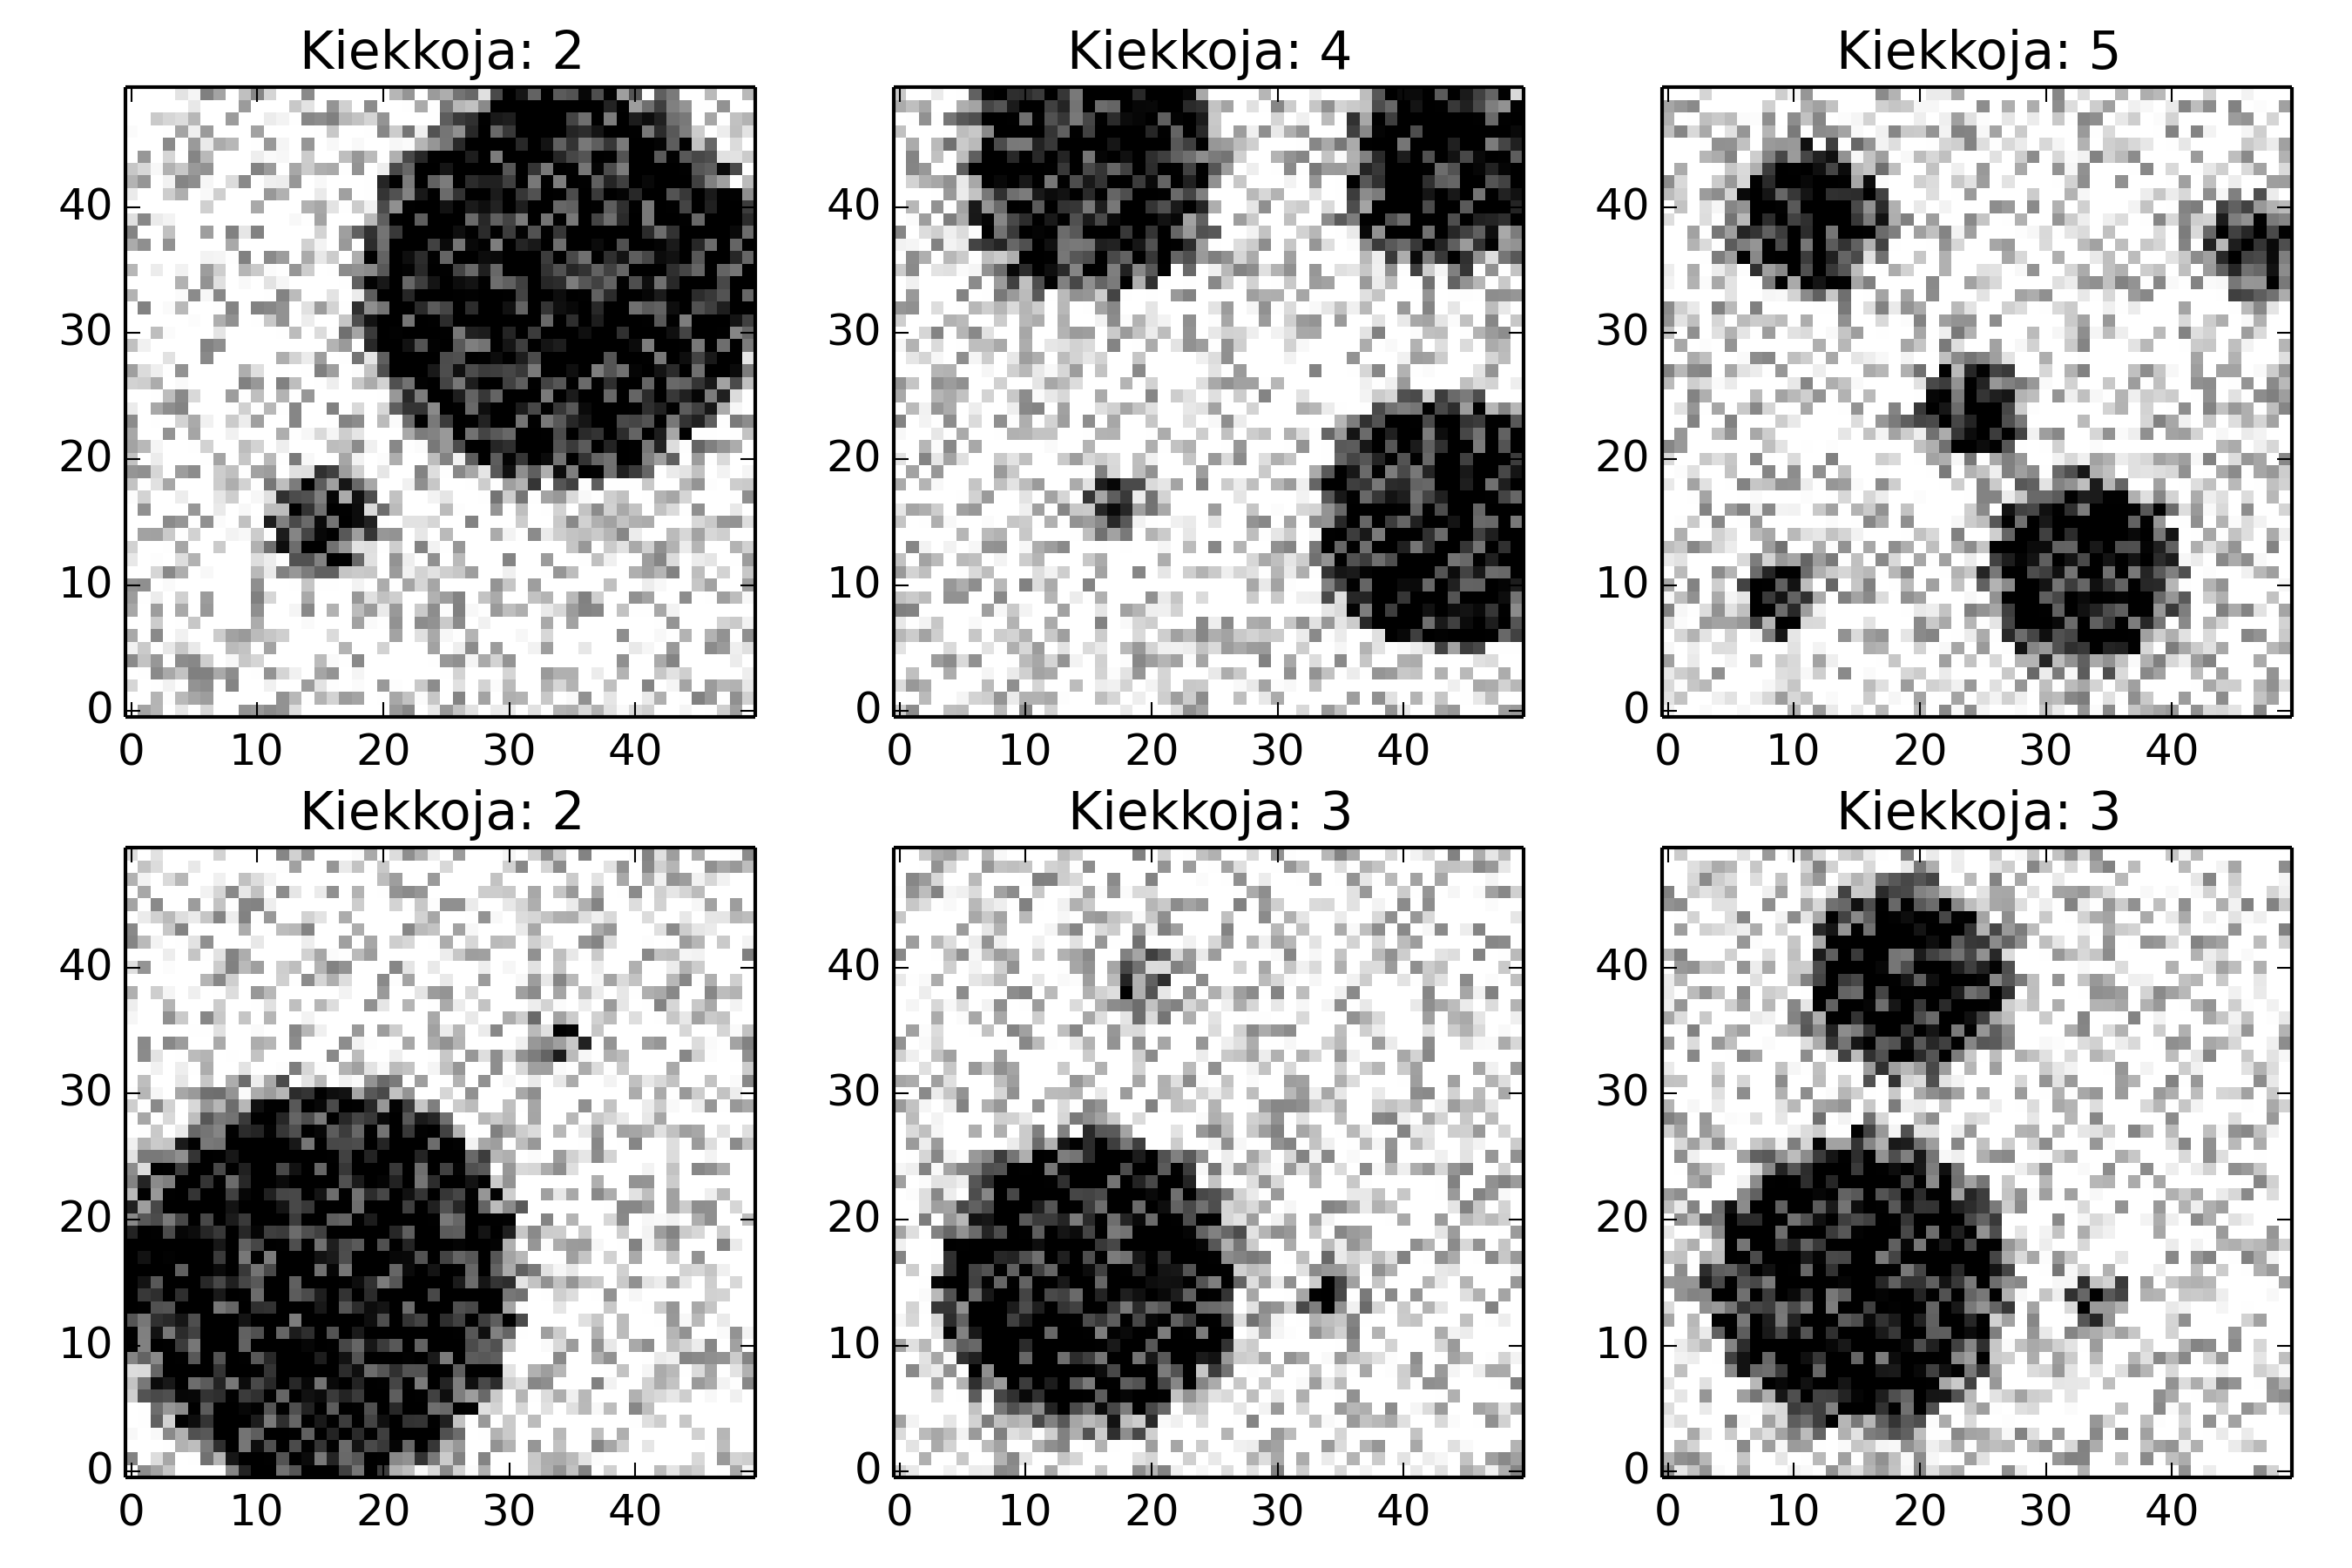
\includegraphics[width=\linewidth]{figures/all_datasets.png}
    \caption{Tutkielmassa lähemmin tarkasteltavat testikuvat.
        Vasemmalta oikealle, ylärivi: Testikuvat a, b, c.
        Alarivi: d, e, f.
    \label{fig:all_datasets}}
\end{figure}

\section{Ratkaisun onnistumisen mittaaminen}
\label{sec:ratkaisun_onnistumisen_mittaaminen}

Kuvaillaan vielä mitat, joita käytetään ratkaisun onnistumisen arvioimiseen.

\subsection{Energiafunktio}
\label{sub:energiafunktio}

Energiafunktion arvon tarkastelu kullakin iteraatiolla kunkin kulkijan edetessä on luonnollinen menetelmä arvioida optimointialgoritmin toimintaa.
Varjopuolena kuva energiafunktion tarkastelu ei välttämättä kerro paljonkaan kuinka hyvä ratkaisu on tarkasteltavan kuvakäsittelyongelman suhteen.

\subsection{Pinta-alan symmetrinen erotus}
\label{sub:pinta_alan_symmetrinen_erotus}

Toinen vaihtoeheto on verrata todellisen ja ratkaisun kiekkojen symmetristä erotusta.
Olkoon $W_\text{final}$ kulkijan lopullinen ratkaisu ympyräparametreille ja $W_\text{orig}$ alkuperäiset datan luomiseen käytetyt kiekkojen parametrit,
ja $A_W$ luvun~\ref{cha:kuvamalli_ja_aineisto} mallin mukaisesti kiekkoparametreja vastaava häiriötön kuva jossa $A_{ij} = 0$, jos pikseli on kuvan sisällä.
Olkoon myös vastaava kuvaa $A$ vastaava käänteiskuva $A' = 1 - A$ kuten kappaleessa~\ref{sub:paranneltu_monen_kiekon_energiafunktio}.
Tälloin symmetriseen erotukseen perustuva mitta on
\begin{equation*}
    m_\text{symm}(W_\text{final}, W_\text{orig}) = (A_{W_\text{final}}' \setminus A_{W_\text{orig}}') \cup (A_{W_\text{orig}}' \setminus A_{W_\text{final}}'),
\end{equation*}
kun kuvamatriisit mielletään joukoiksi, johon joku tietty pikseli kuuluu ($A_{ij}' = 1$) tai ei ($A_{ij}' = 0$).
Mitta vastaa naiivia energiafunktiota ja melko samankaltainen parannellun energiafunktion kanssa.

\subsection{Sovellettu etäisyysmitta}
\label{sub:sovellettu_etaisyysmitta}

Määritellään lisäksi toisenlainen ratkaisukiekkojen etäisyyttä todellisista mittaava mitta joka ei perustu pinta-aloihin,
mutta kuitenkin vastaa intuitiivisista käsitystä kiekkojen etäisyydestä:
Valitaan löydetyn ratkaisun ja todellisten kiekkojen väliseksi etäisyydeksi summa kunkin ratkaisukiekon keskipisteen ja säteen Euklidinen etäisyys alkuperäisten kiekkojen keskipisteeseen ja säteeseen
kun ratkaisun kiekkojen todelliset vastineet valitaan kaikkien mahdollisten kiekkoparien etäisyyksien pienuusjärjestyksessä.

Toisin sanoen käytetään seuraavanlaista algoritmia.
Olkoon $W_\text{final}, W_\text{orig}$  kiekkojoukot kuten yllä, ja lasketaan etäisyys $m_\text{sov}$ seuraavasti:
\begin{algorithm}[h]
    \KwData{$W_\text{final}, W_\text{orig}$}
    \KwResult{$m_\text{sov}$}
    \BlankLine
    $n_\text{circles} \leftarrow \abs{W}$ \;
    $m_s \leftarrow 0$\;
    \For{$i \leftarrow 1$ \KwTo $n_\text{circles}$}{
        $d_\text{min} \leftarrow \min\limits_{a \in W_\text{final}, b \in W_\text{orig}} \norm{a.x - b.y} + \norm{a.y - b.y} + \norm{a.r - b.r}$\;
        $a_\text{min}, b_\text{min} \leftarrow \underset{a \in W_\text{final}, b \in W_\text{orig}}{\operatorname{argmin}} \norm{a.x - b.y} + \norm{a.y - b.y} + \norm{a.r - b.r}$\;
        $m_\text{sov} \leftarrow m_s + d_\text{min}$\;
        $W_\text{final} \leftarrow W_\text{final} \setminus a_\text{min}$\;
        $W_\text{orig} \leftarrow W_\text{orig} \setminus b_\text{min}$\;
    }
\end{algorithm}


\section{Algoritmin tulokset}
\label{sec:algoritmin_tulokset}

Testiaineiston kuville ajettiin 100 kertaa luvussa~\ref{cha:algoritmin_soveltaminen} kuvailtu algoritmi vaihtelevalla määrällä jäähdytysskenaarioita $\alpha = 0.90 \dots 0.99$.
Jokaista algoritmin ajokertaa tietyin parametrein eli toteutunutta Markov-ketjua nimitetään jatkossa \emph{kulkijaksi}.

Koska kulkijat ovat itsenäisiä, kunkin 100 kulkijan kokoelman simuloinnissa voitiin hyödyntää rinnakkaislaskentaa.
Numeeriseen laskentaan käytettiin Helsingin yliopiston Tietojenkäsittelytieteen laitoksen Ukko-laskentaklusteria.

\begin{table}[htpb]
    \centering
    \caption{Testiaineiston kuvat a, b, c. Kuvien~\ref{fig:A_datasets_res_fast} ja \ref{fig:A_datasets_res_slow} energiafunktion suhteen parhaiden ratkaisujen lopulliset energiat, virheet ja kulkijoiden pituus (homogeenien Markov-ketjujen määrä). Jäähdytysskenaariot $\alpha = 0.90$ ja $\alpha = 0.99$.
        \label{tab:A_res_fast_errors}
    }
    \begin{tabular}{l c c c c c}
        $\alpha$ & Aineisto & Markov-ketjuja & Energia & $m_\text{sov}$ & $m_\text{symm}$ \\[2pt]
        \hline\noalign{\smallskip}
        0.90 & a & 56 & 129.982734083 & 1.43765180533 & 22 \\
             & b & 52 & 136.670018567 & 3.36654077973 & 66 \\
             & c & 60 & 159.514844916 & 6.75832581266 & 131 \\[1pt]
        \hline\noalign{\smallskip}
        0.99 & a & 679 & 129.277573595 & 1.41934200707 & 22\\
             & b & 411 & 135.156720071 & 5.0613981837 & 49\\
             & c & 438 & 149.503374454 & 27.974956417 & 73
    \end{tabular}
\end{table}

\begin{figure}[htpb]
    \centering
    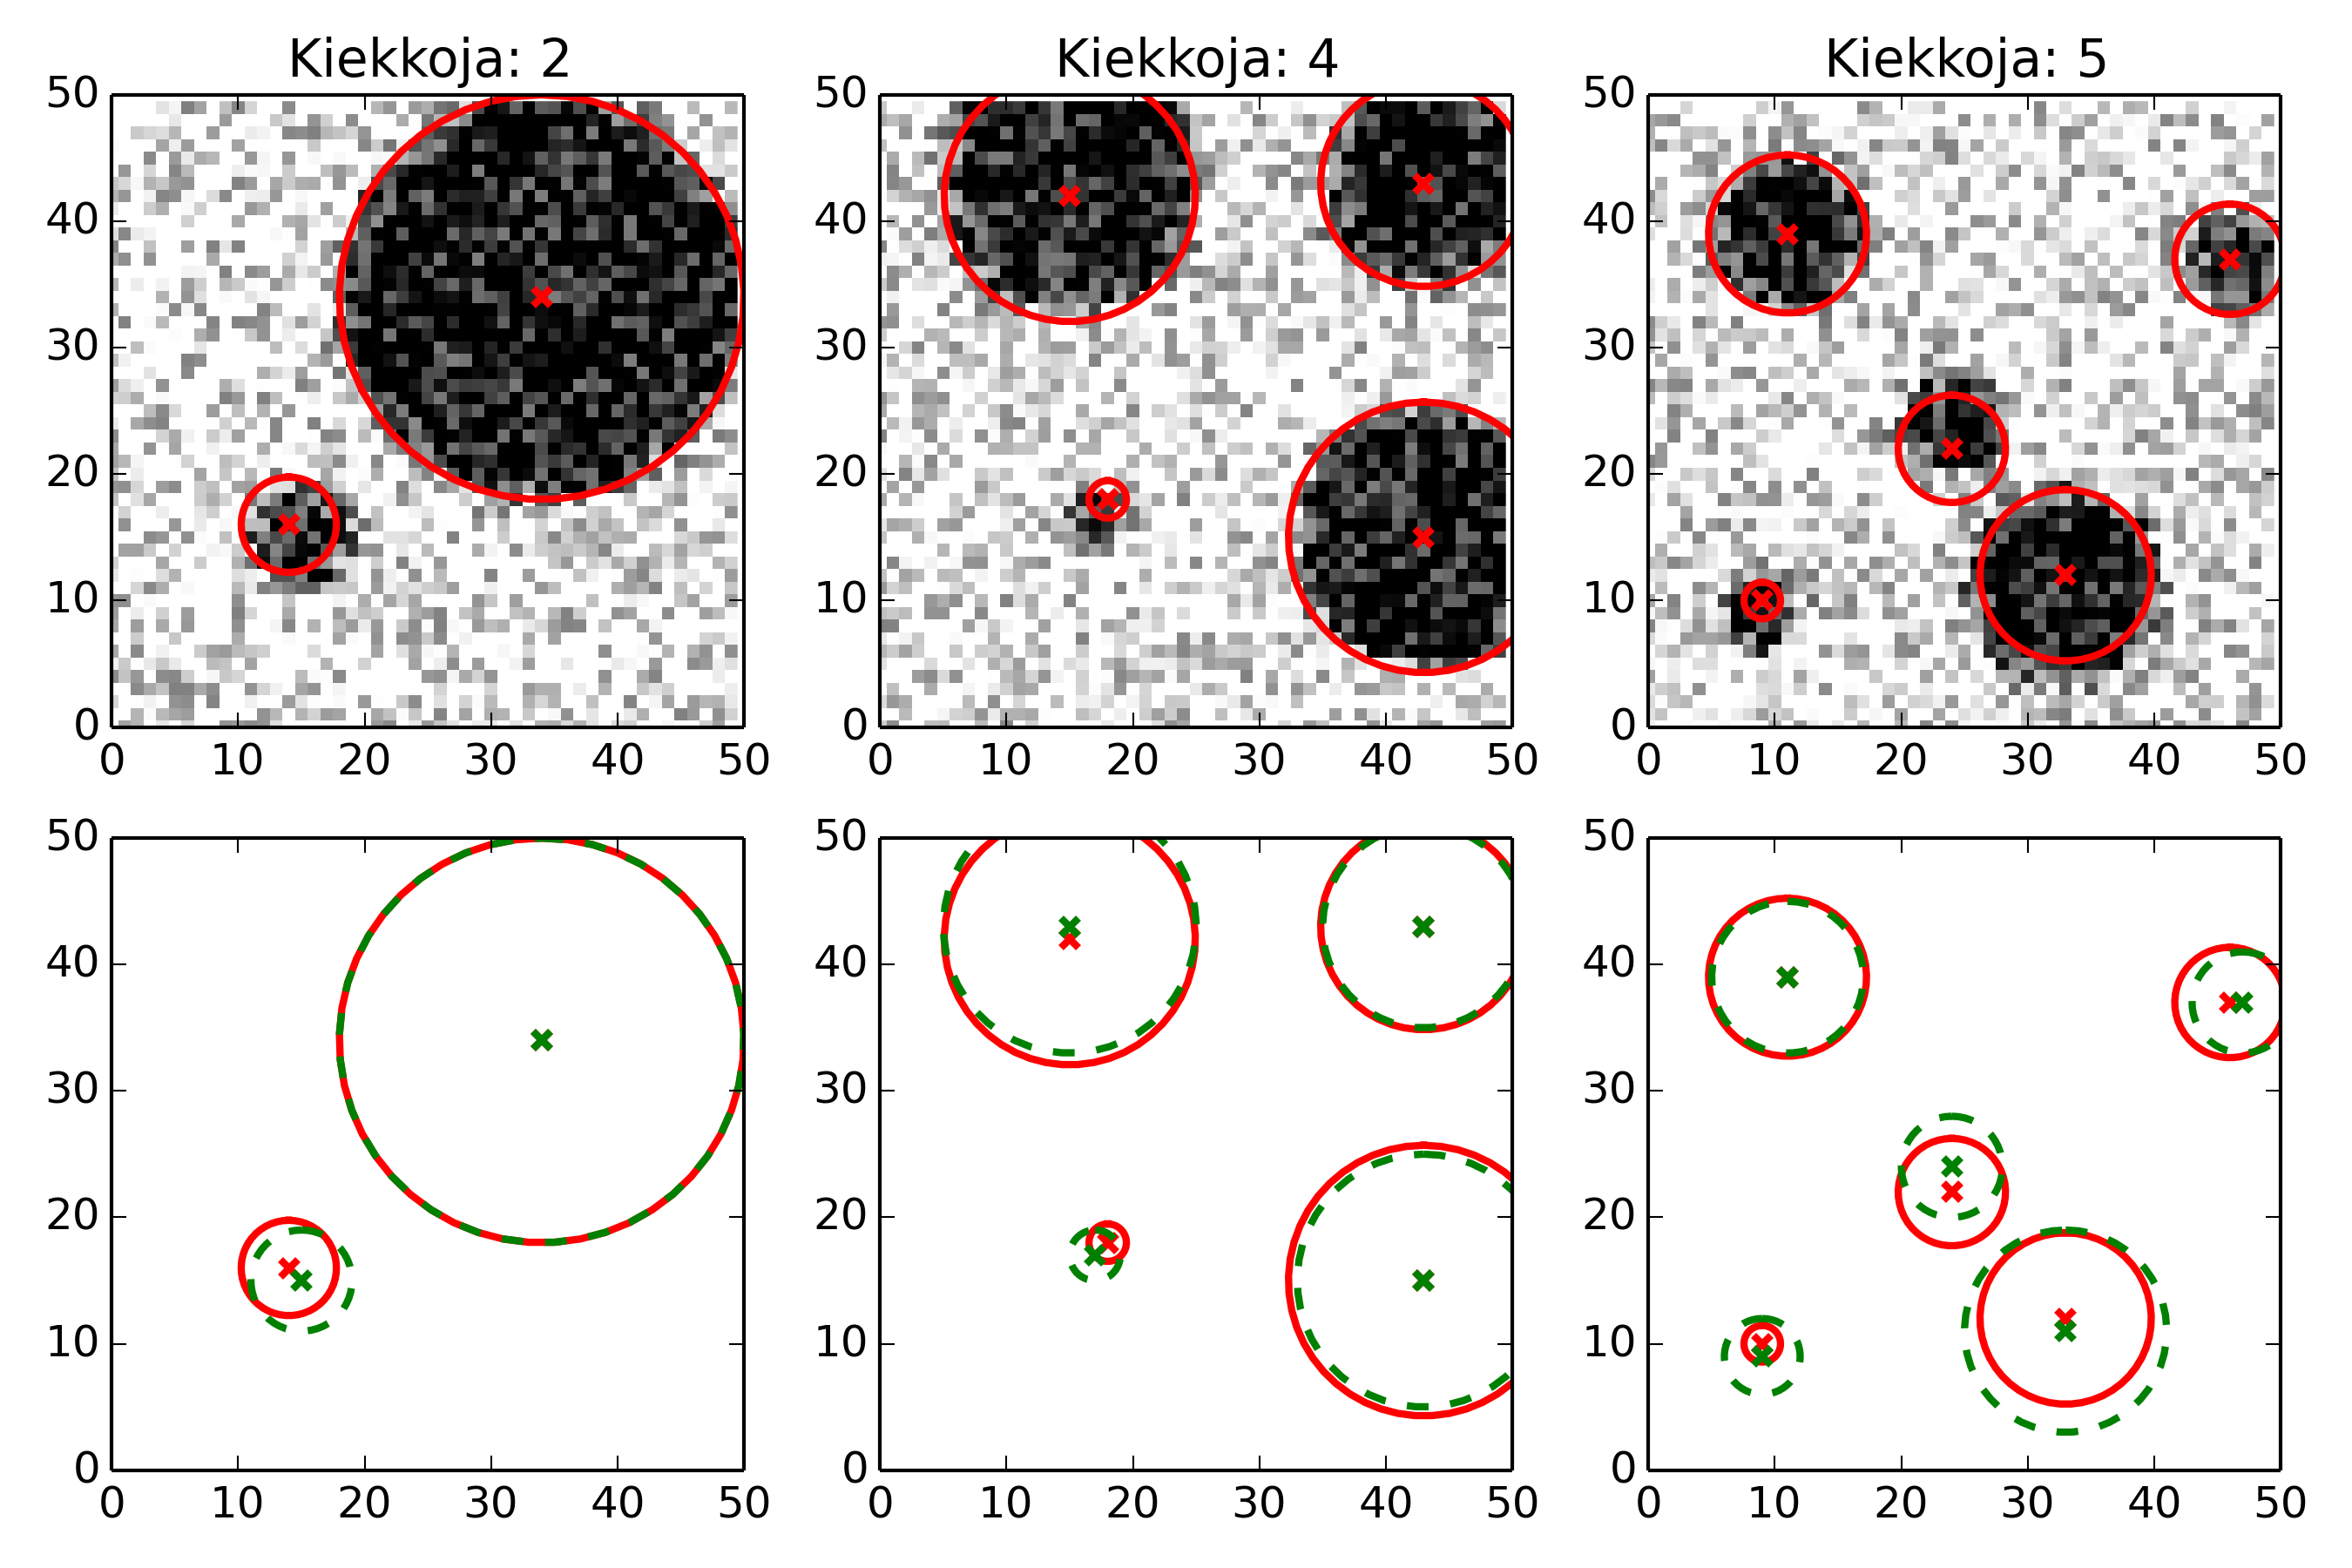
\includegraphics[width=1.0\linewidth]{figures/A_datasets_res_fast.png}
    \caption{Testiaineiston kuvat a, b, c: Parhaat ratkaisut energiafunktion suhteen (punaiset ympyrät) 100 kulkijan kokoelmasta jäähdytysskenaariolla $\alpha = 0.90$.
        Todelliset kiekot alarivillä vihreällä katkoviivalla.
        \label{fig:A_datasets_res_fast}
    }
\end{figure}


\begin{figure}[htpb]
    \centering
    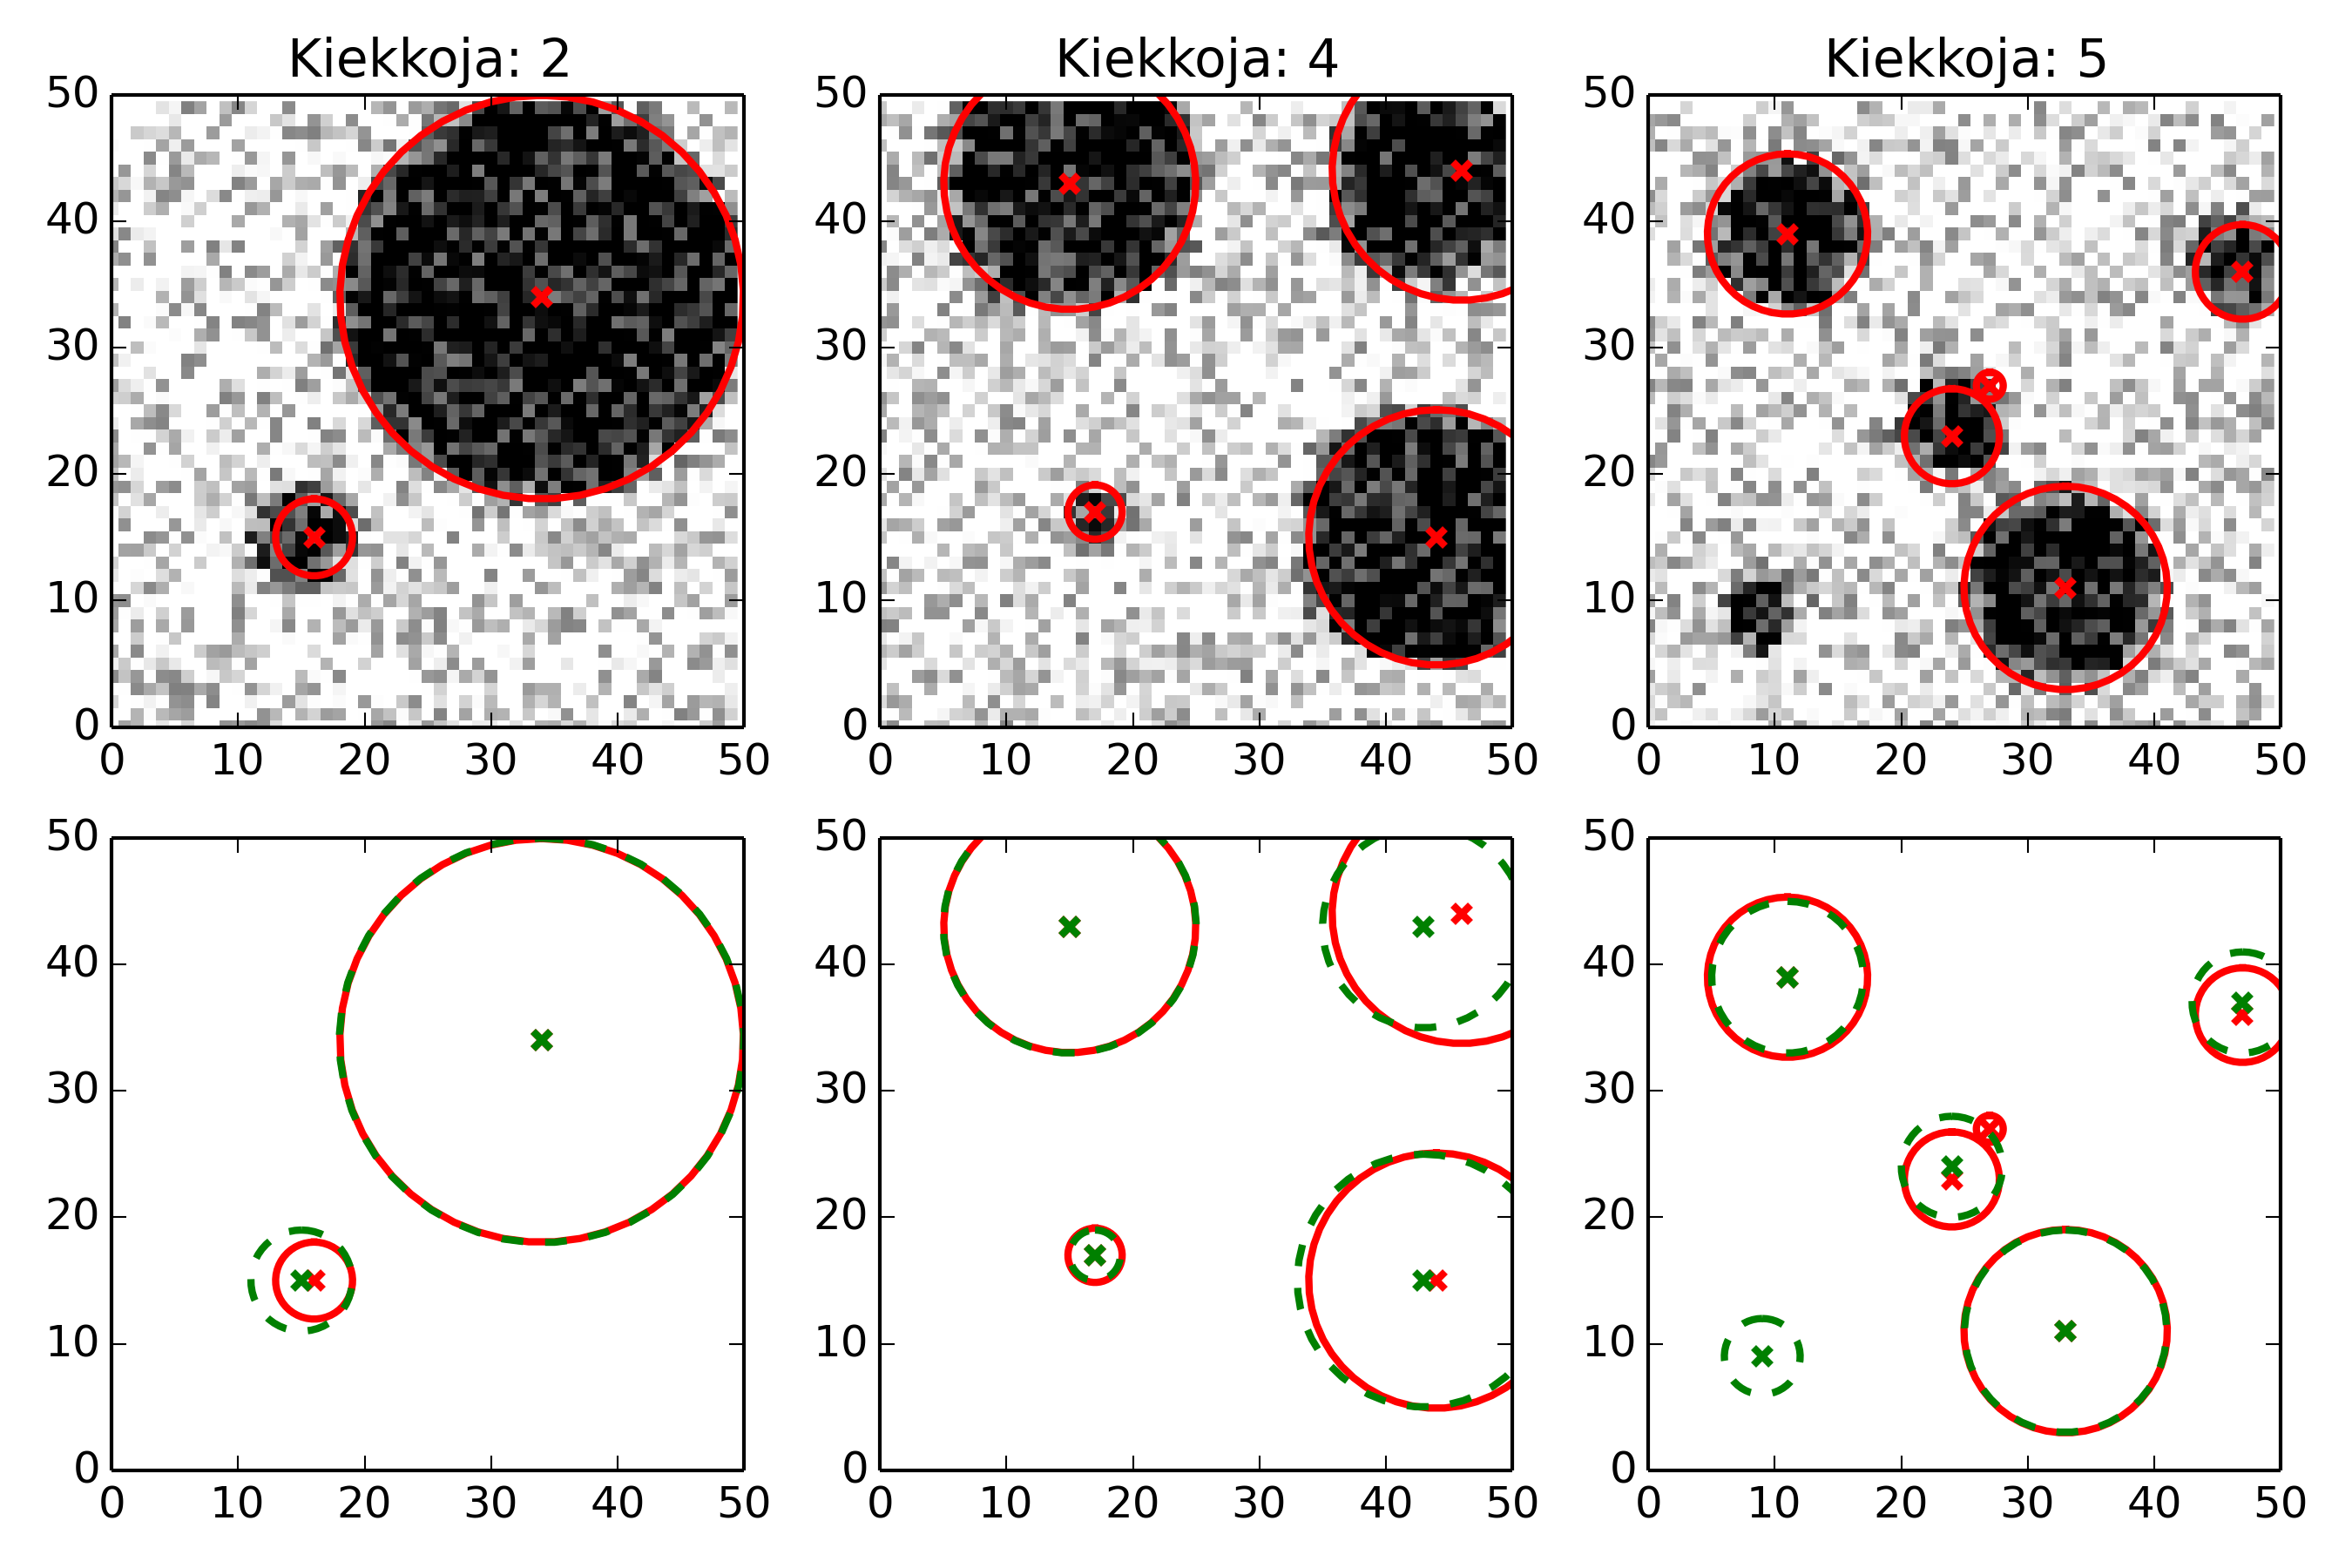
\includegraphics[width=1.0\linewidth]{figures/A_datasets_res_slow.png}
    \caption{Samat testikuvat a, b, c kuin kuvassa~\ref{fig:A_datasets_res_fast}: Parhaat ratkaisut energiafunktion suhteen (punaiset ympyrät) 100 kulkijan kokoelmasta jäähdytysskenaariolla $\alpha = 0.99$.
        \label{fig:A_datasets_res_slow}
    }
\end{figure}

\begin{figure}[htpb]
    \centering
    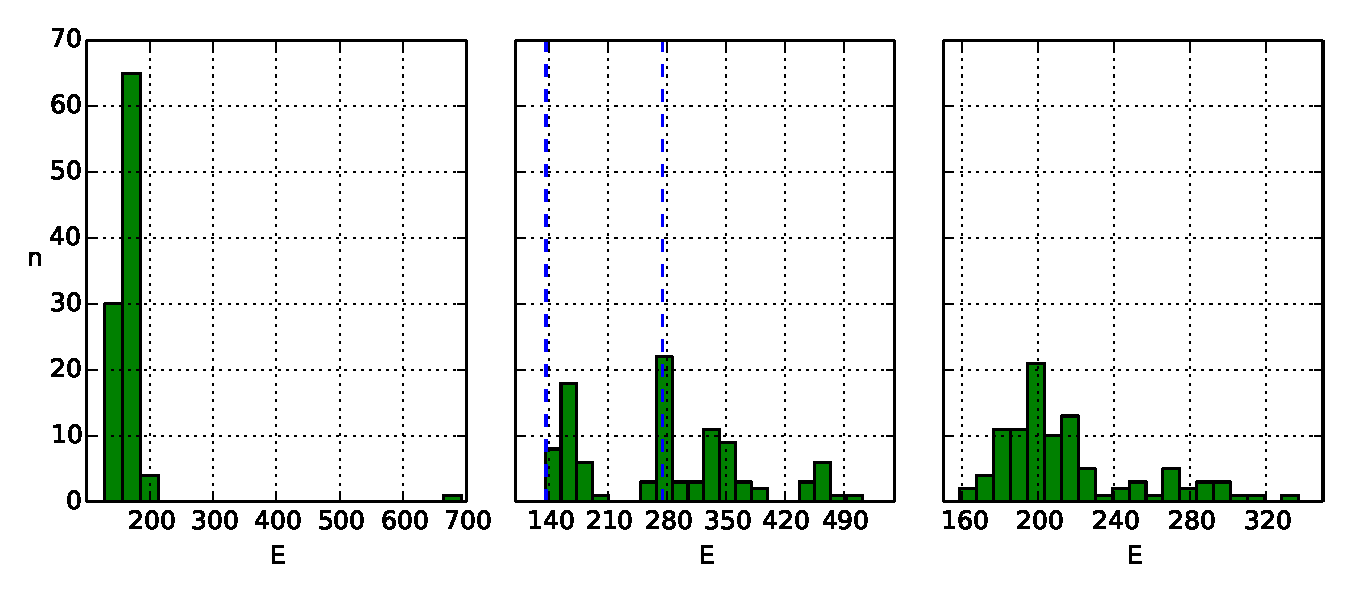
\includegraphics[width=1.0\linewidth]{figures/A_final_histo3_fast.pdf}
    \caption{Kuvan~\ref{fig:A_datasets_res_fast} skenaariota vastaavien kokoelmien kulkijoiden lopullisten energioiden jakaumat.
        Testikuvaa b vastaavaan histogrammiin merkitty kokoelman energialtaan paras ratkaisu sekä histogrammin moodi ($E \approx 280$).
        \label{fig:A_final_histo3_fast}
    }
\end{figure}


\begin{figure}[htpb]
    \centering
    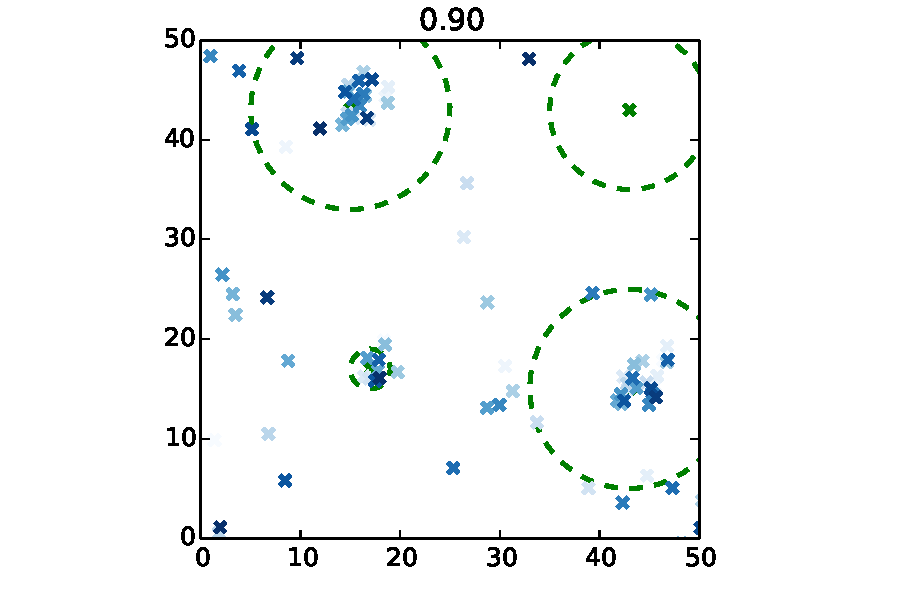
\includegraphics[width=1.0\linewidth]{figures/A_modalbin_cc_fast_1.pdf}
    \caption{Kuvan~\ref{fig:A_final_histo3_fast} testikuvan b histogrammin energiamoodin kulkijoiden ($n = 22$ kpl) löytämät keskipisteet, saman kulkijan pisteet samalla värillä.
        Keskipisteiden sijaintiin lisätty $U(-2,2)$-tärinää päällekkäisten merkkien näkemiseksi.
        Toisin kuin kuvassa~\ref{fig:A_final_histo3_fast} näkyvässä parhaassa ratkaisussa, loppuenergiamoodin kulkijat eivät näytä löytävän neljättä kiekkoa ($x = 44, y = 44, r = 8$).
        \label{fig:A_modalbin_cc_fast_1}
    }
\end{figure}

\begin{table}[htpb]
    \centering
    \caption{Testiaineiston kuva d. Kuvien~\ref{fig:set2_datasets_res_99} -- \ref{fig:set2_datasets_res_90} energiafunktion suhteen parhaiden ratkaisujen lopulliset energiat, virheet ja kulkijoiden pituus.
        \label{tab:2_res_errors}
    }
    \begin{tabular}{l c c c c c}
        Aineisto & $\alpha$ & Markov-ketjuja & Energia & $m_\text{sov}$ & $m_\text{symm}$ \\[2pt]
        \hline\noalign{\smallskip}
        d & 0.99 & 582 & 112.70531642  & 1.34903737042 & 12 \\
          & 0.98 & 292 & 115.799173967 & 17.1400032558 & 20 \\
          & 0.96 & 188 & 113.108609169 & 1.33302834307 & 12 \\
          & 0.94 & 103 & 112.772445287 & 1.3089734381  & 12 \\
          & 0.90 & 70  & 115.694414615 & 33.8856144998 & 22 \\
    \end{tabular}
\end{table}

\begin{figure}[p]
    \centering
    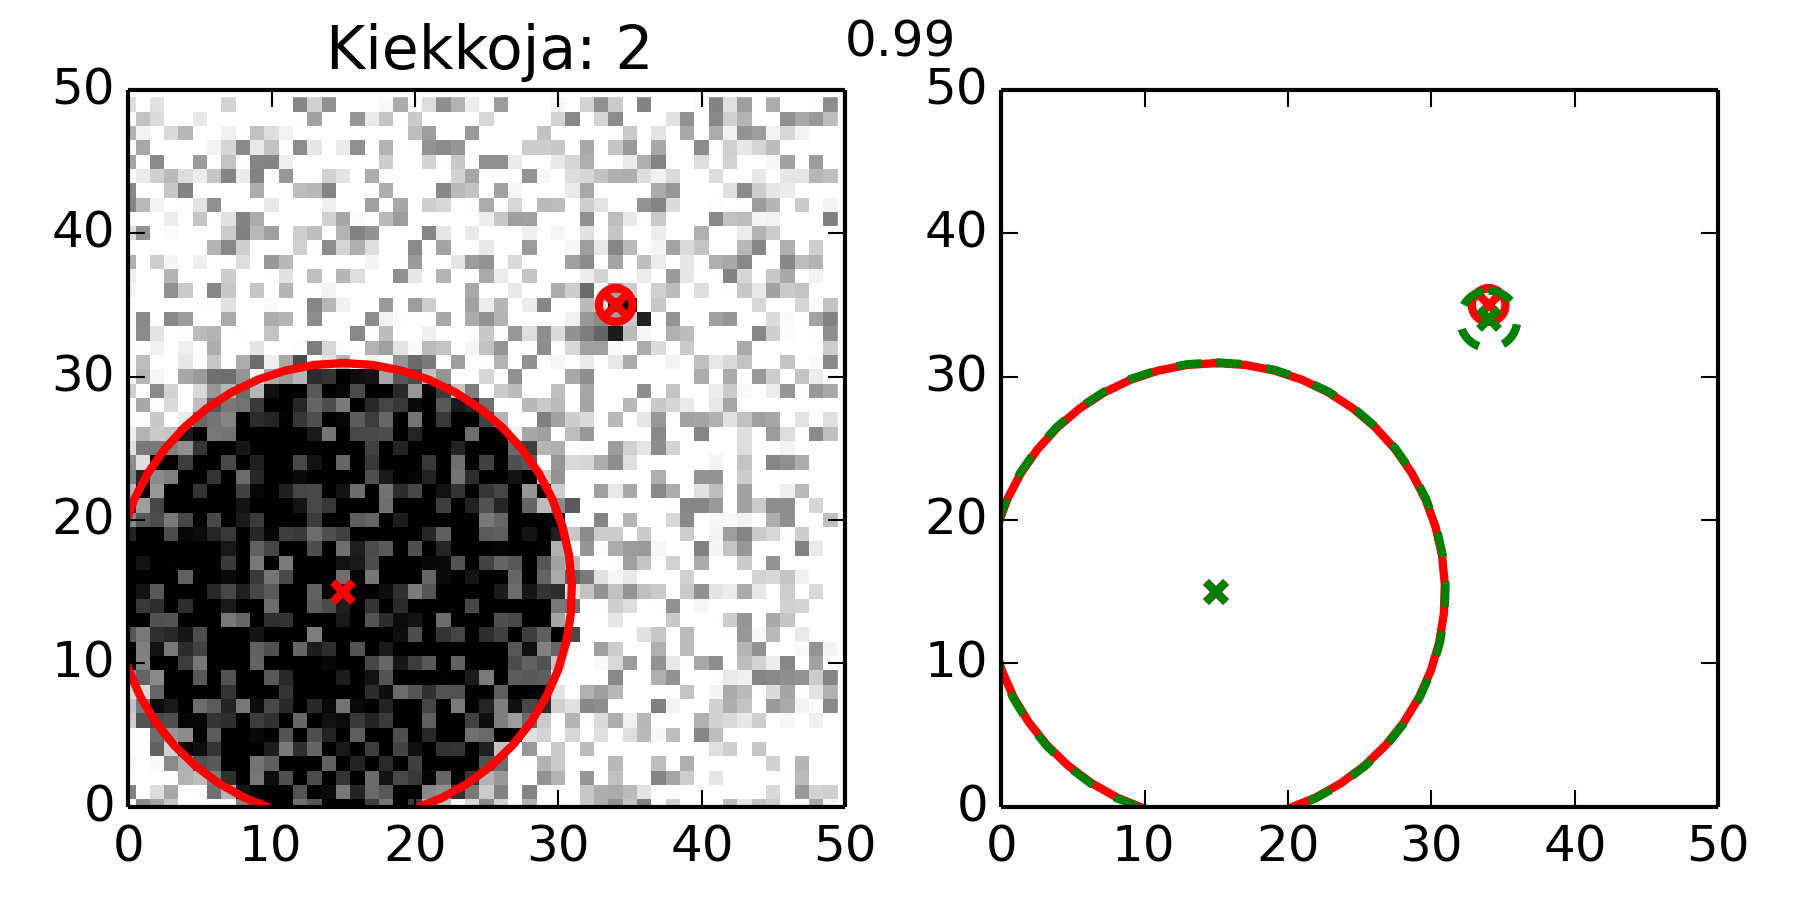
\includegraphics[width=0.7\linewidth]{figures/set2_datasets_res_99.png}
    \caption{Testikuva d, loppuenergialtaan paras kulkija 100 kulkijan kokoelmasta, kun $\alpha = 0.99$.
        \label{fig:set2_datasets_res_99}
    }
\end{figure}

\begin{figure}[p]
    \centering
    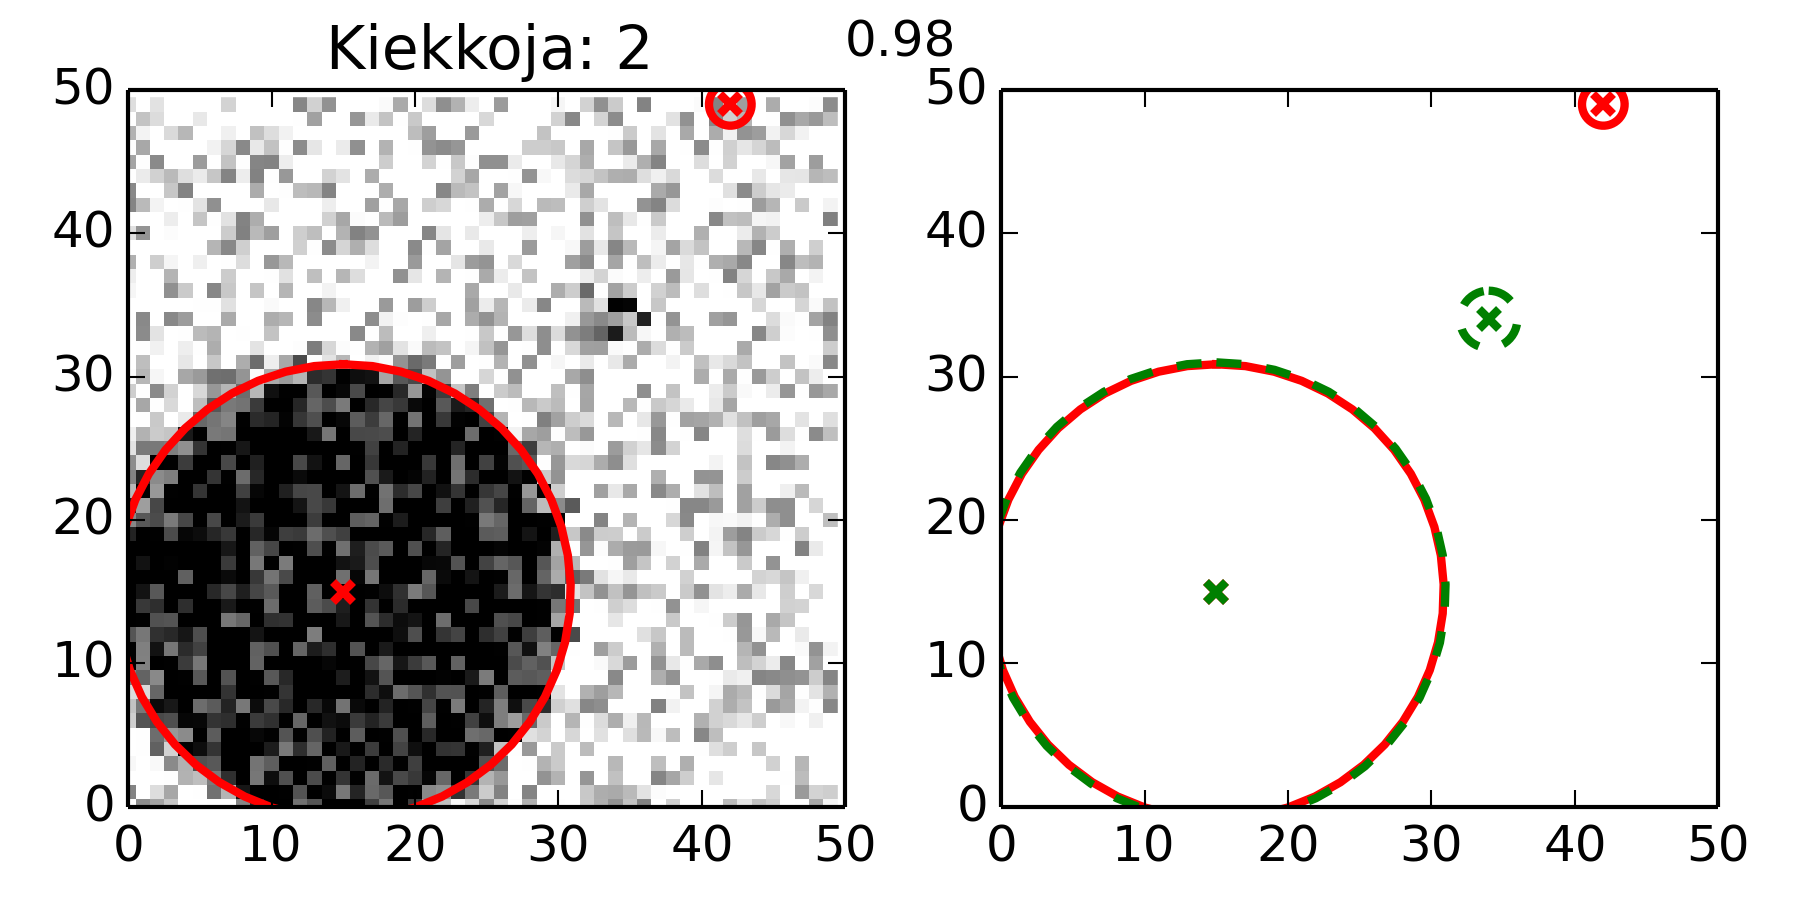
\includegraphics[width=0.7\linewidth]{figures/set2_datasets_res_98.png}
    \caption{Testikuva d. $\alpha = 0.98$.
        \label{fig:set2_datasets_res_98}
    }
\end{figure}


\begin{figure}[p]
    \centering
    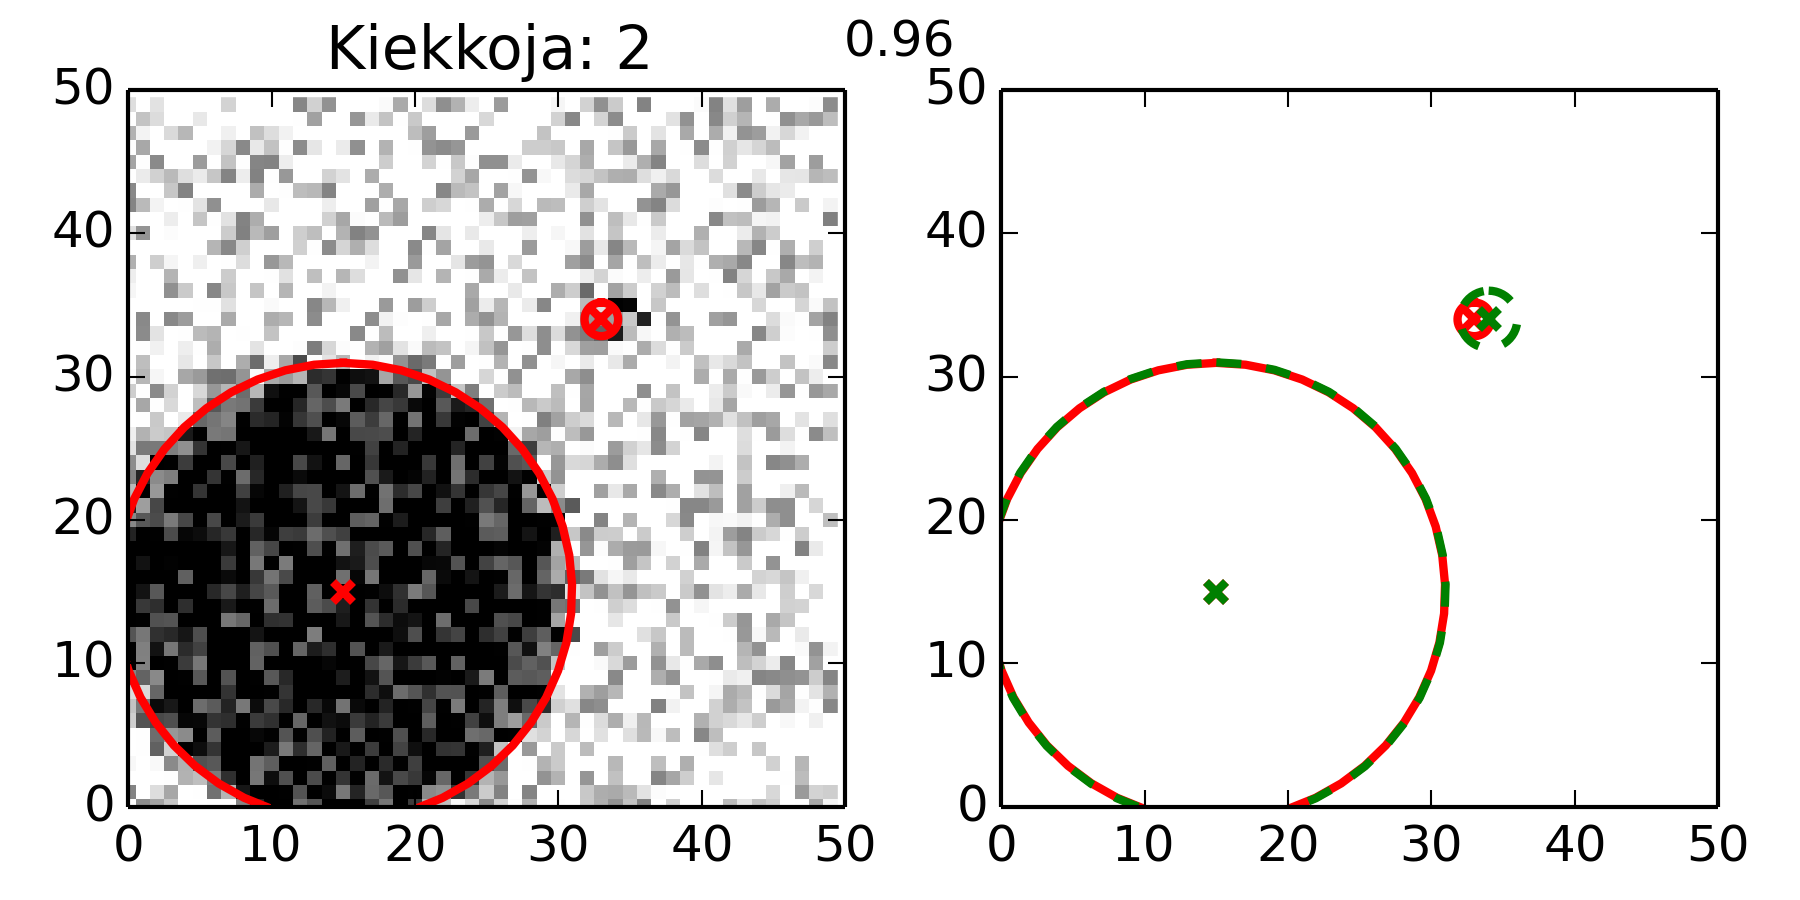
\includegraphics[width=0.7\linewidth]{figures/set2_datasets_res_96.png}
    \caption{Testikuva d. $\alpha = 0.96$.
        \label{fig:set2_datasets_res_96}
    }
\end{figure}


\begin{figure}[p]
    \centering
    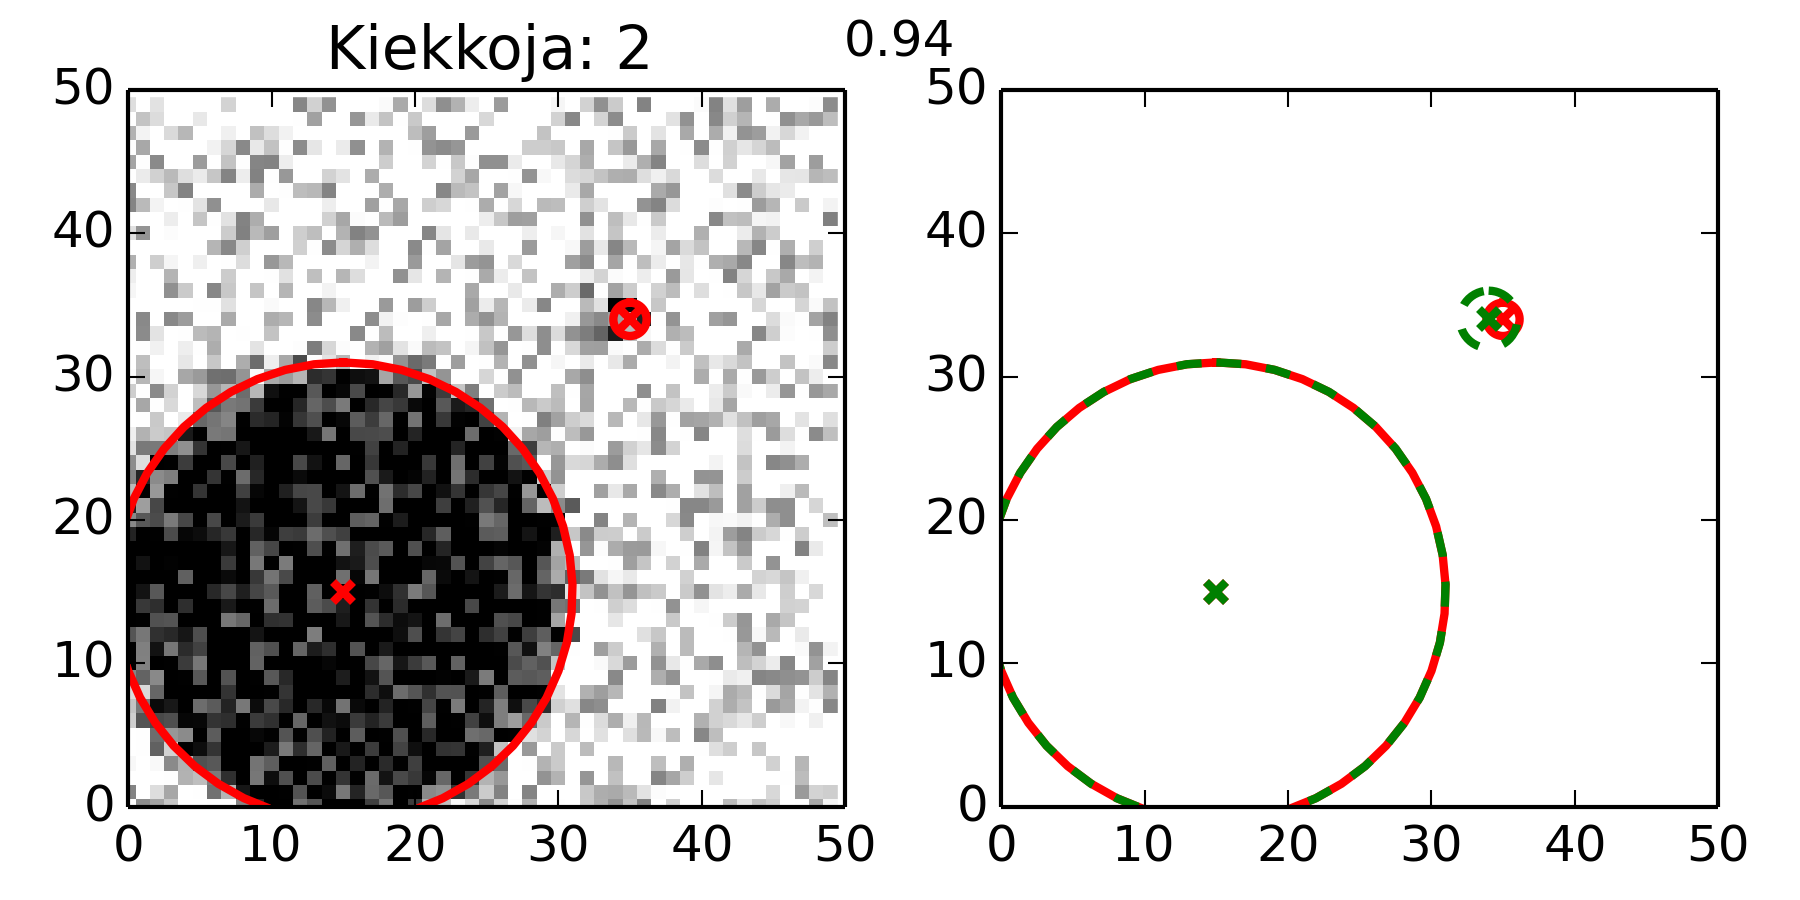
\includegraphics[width=0.7\linewidth]{figures/set2_datasets_res_94.png}
    \caption{Testikuva d. $\alpha = 0.94$.
        \label{fig:set2_datasets_res_94}
    }
\end{figure}


\begin{figure}[p]
    \centering
    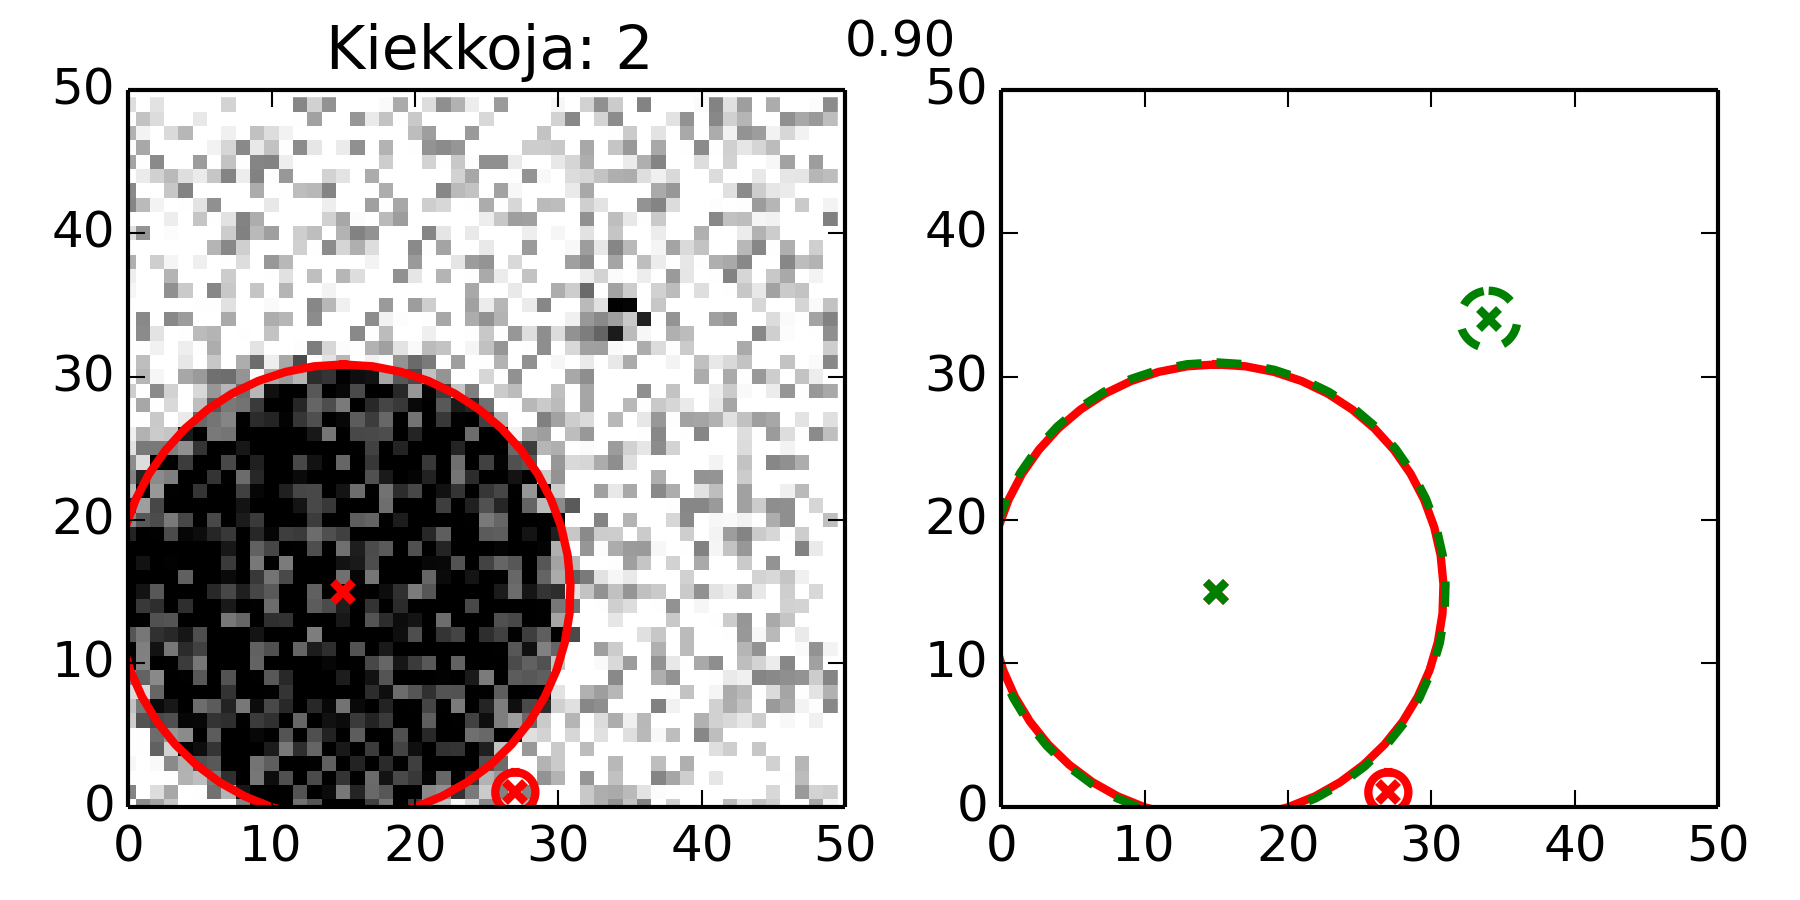
\includegraphics[width=0.7\linewidth]{figures/set2_datasets_res_90.png}
    \caption{Testikuva d. $\alpha = 0.90$.
        \label{fig:set2_datasets_res_90}
    }
\end{figure}

\begin{figure}[p]
    \centering
    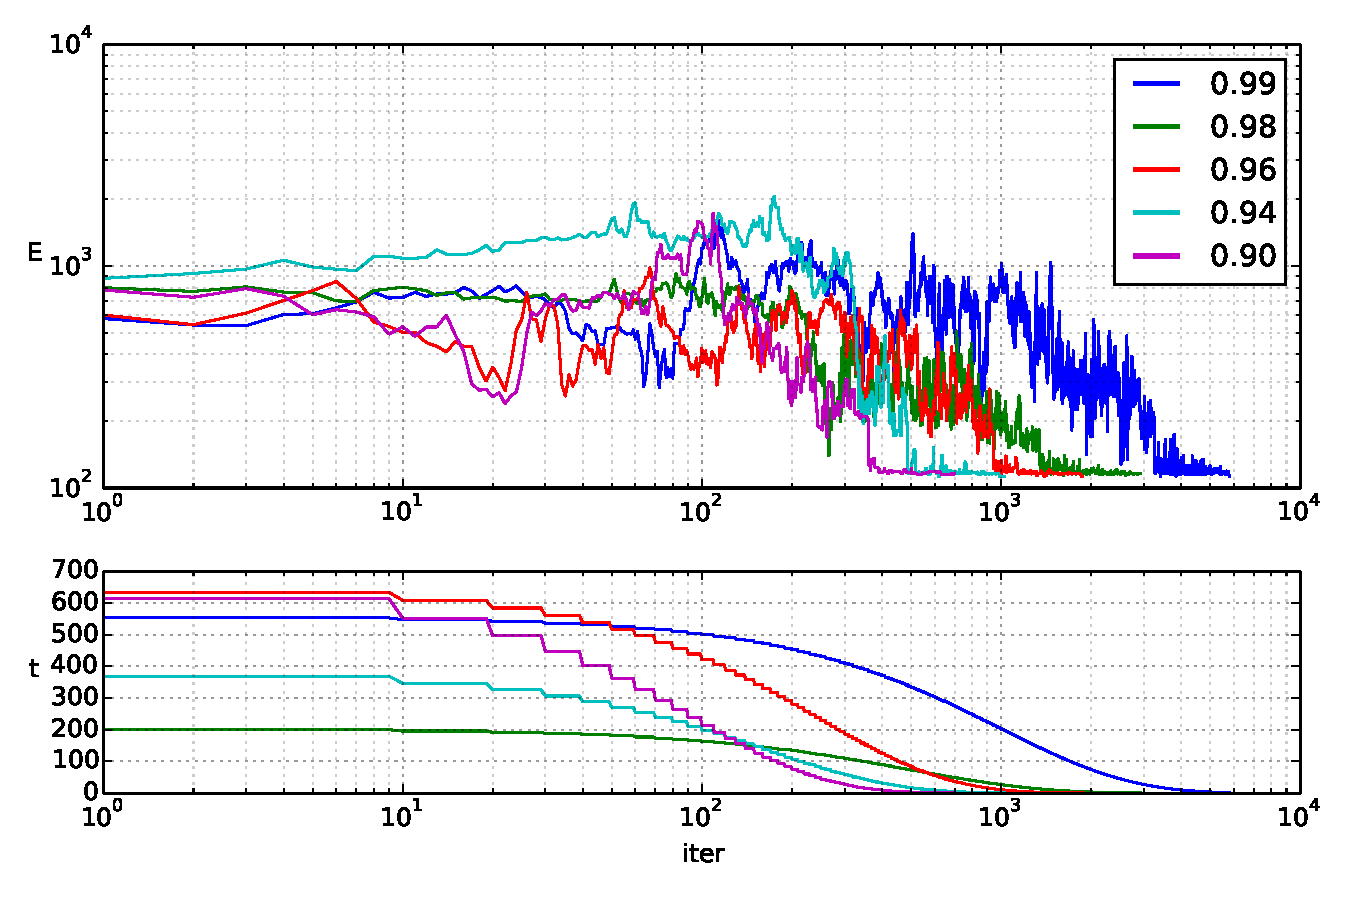
\includegraphics[width=1\linewidth]{figures/set2_walkers_temp.pdf}
    \caption{
        Kuvien \ref{fig:set2_datasets_res_99} -- \ref{fig:set2_datasets_res_90} kulkijoiden energioiden ja lämpötilojen kehitys.
        Stokastisen alkuarvon asetuksen takia alkulämpötilassa on huomattavaa vaihtelua ($t_0 \approx 200 \dots 700$).
        \label{fig:set2_walkers_temp}
    }
\end{figure}

\begin{figure}[p]
    \centering
    \makebox[\textwidth][c]{
        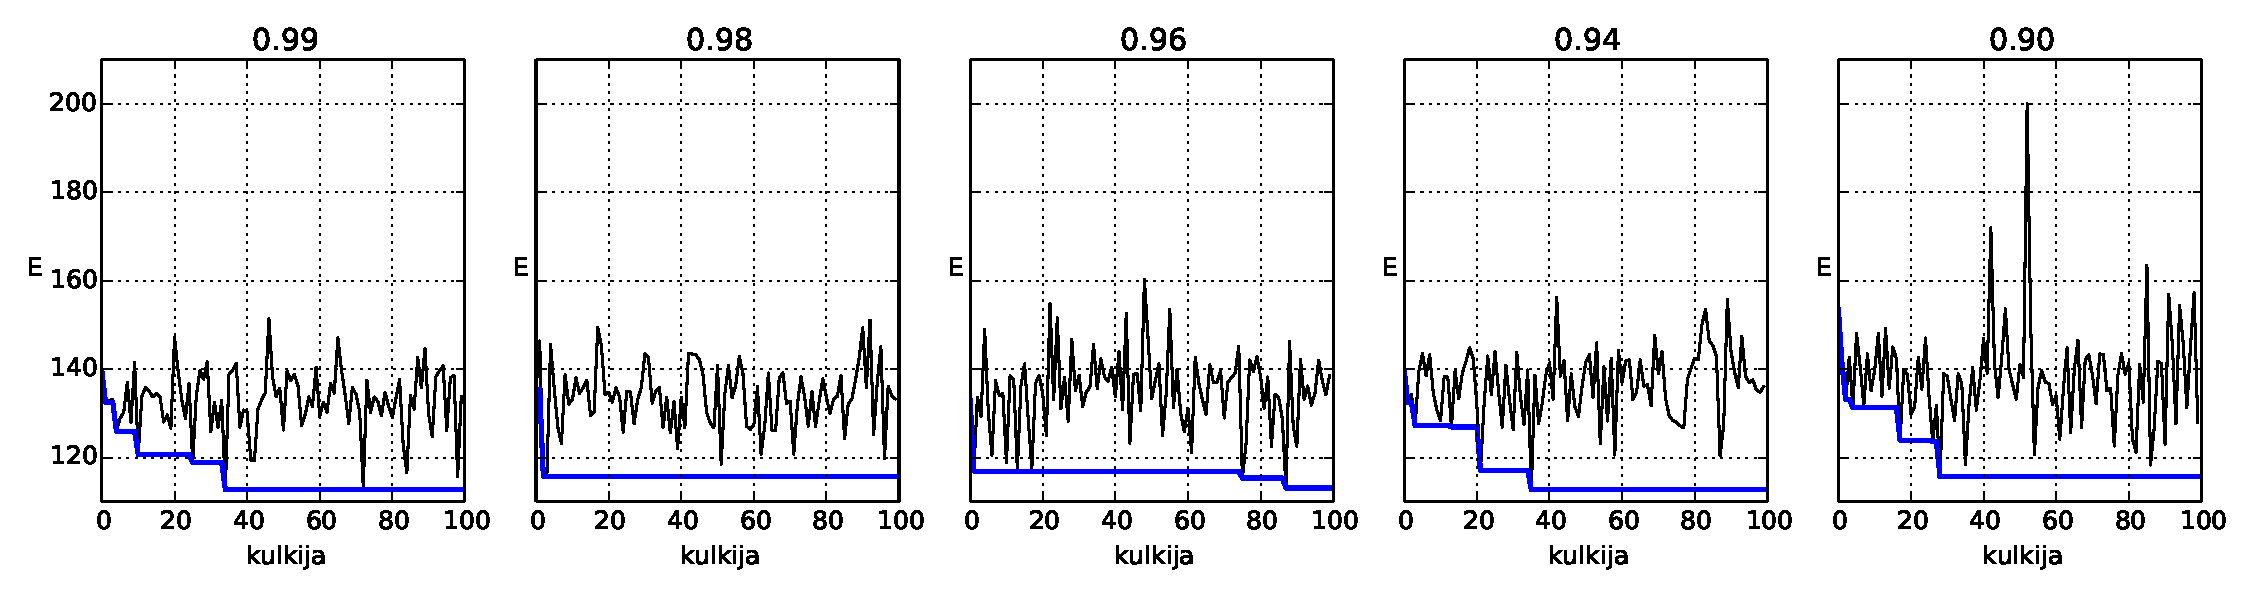
\includegraphics[width=1.4\linewidth]{figures/set2_best_final_e_walkers.pdf}
    }
    \caption{Kuvien \ref{fig:set2_datasets_res_99} -- \ref{fig:set2_datasets_res_90} vastaavien kokoelmien parhaan energian kehitys kokoelman koon funktiona.
        %Todo. Vastaava rivi histogrammeista?
        \label{fig:set2_best_final_e_walkers}
    }
\end{figure}

\FloatBarrier

\begin{table}[htpb]
    \centering
    \caption{Testiaineiston kuvat e,f. Kuvien~\ref{fig:set3_datasets_res_099} ja \ref{fig:set3_datasets_res_090} energiafunktion suhteen parhaiden ratkaisujen lopulliset energiat, virheet ja kulkijoiden pituus.
        \label{tab:3_res_errors}
    }
    \begin{tabular}{l c c c c c}
        $\alpha$ & Aineisto & Markov-ketjuja & Energia & $m_\text{sov}$ & $m_\text{symm}$ \\[2pt]
        \hline\noalign{\smallskip}
        0.99 & e & 636 & 126.820768777 & 41.7710820974 & 26 \\
             & f & 483 & 131.350277715 & 21.2525820166 & 58 \\[1pt]
        \hline\noalign{\smallskip}
        0.94 & e & 89  & 126.912392409 & 29.5102365738 & 36 \\
             & f & 102 & 134.677587474 & 27.8990164056 & 70 \\[1pt]
        \hline\noalign{\smallskip}
        0.90 & e & 74  & 124.101054568 & 11.8660423496 & 30 \\
             & f & 65  & 139.955257356 & 14.0600416833 & 92
    \end{tabular}
\end{table}

\begin{figure}[htpb]
    \centering
    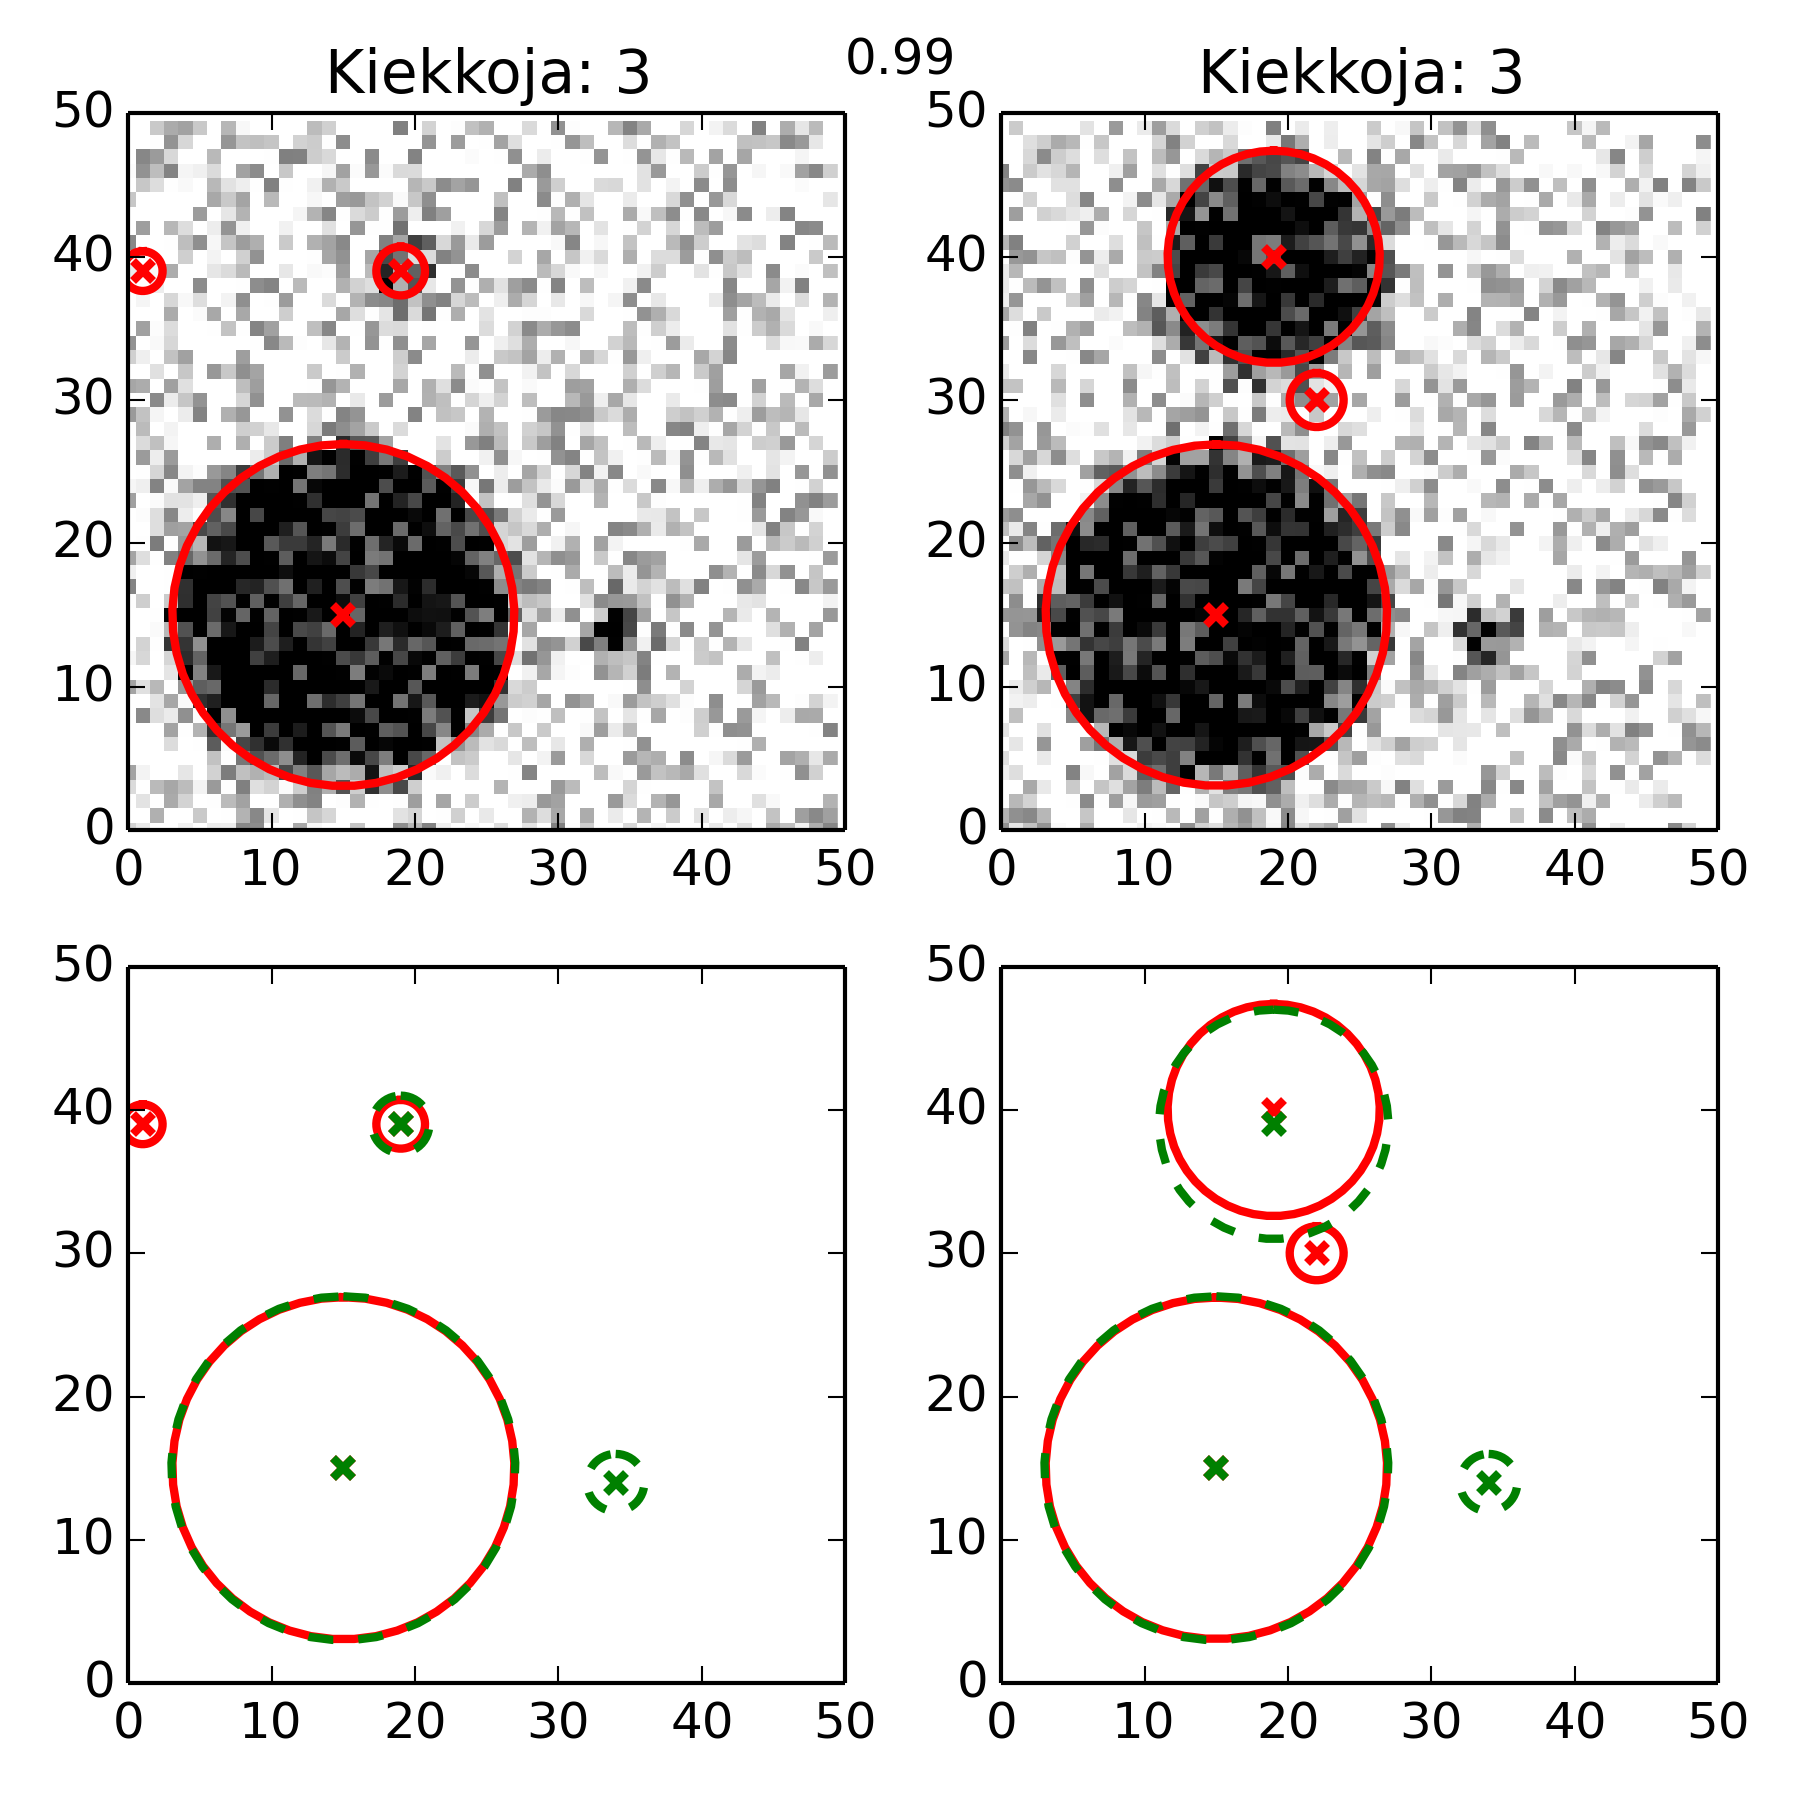
\includegraphics[width=0.7\linewidth]{figures/set3_datasets_res_099.png}
    \caption{
        Kuvat e, f: Parhaat ratkaisut (punaiset ympyrät) 100 kulkijan kokoelmasta jäähdytysskenaariolla $\alpha = 0.99$.
        \label{fig:set3_datasets_res_099}
    }
\end{figure}


\begin{figure}[htpb]
    \centering
    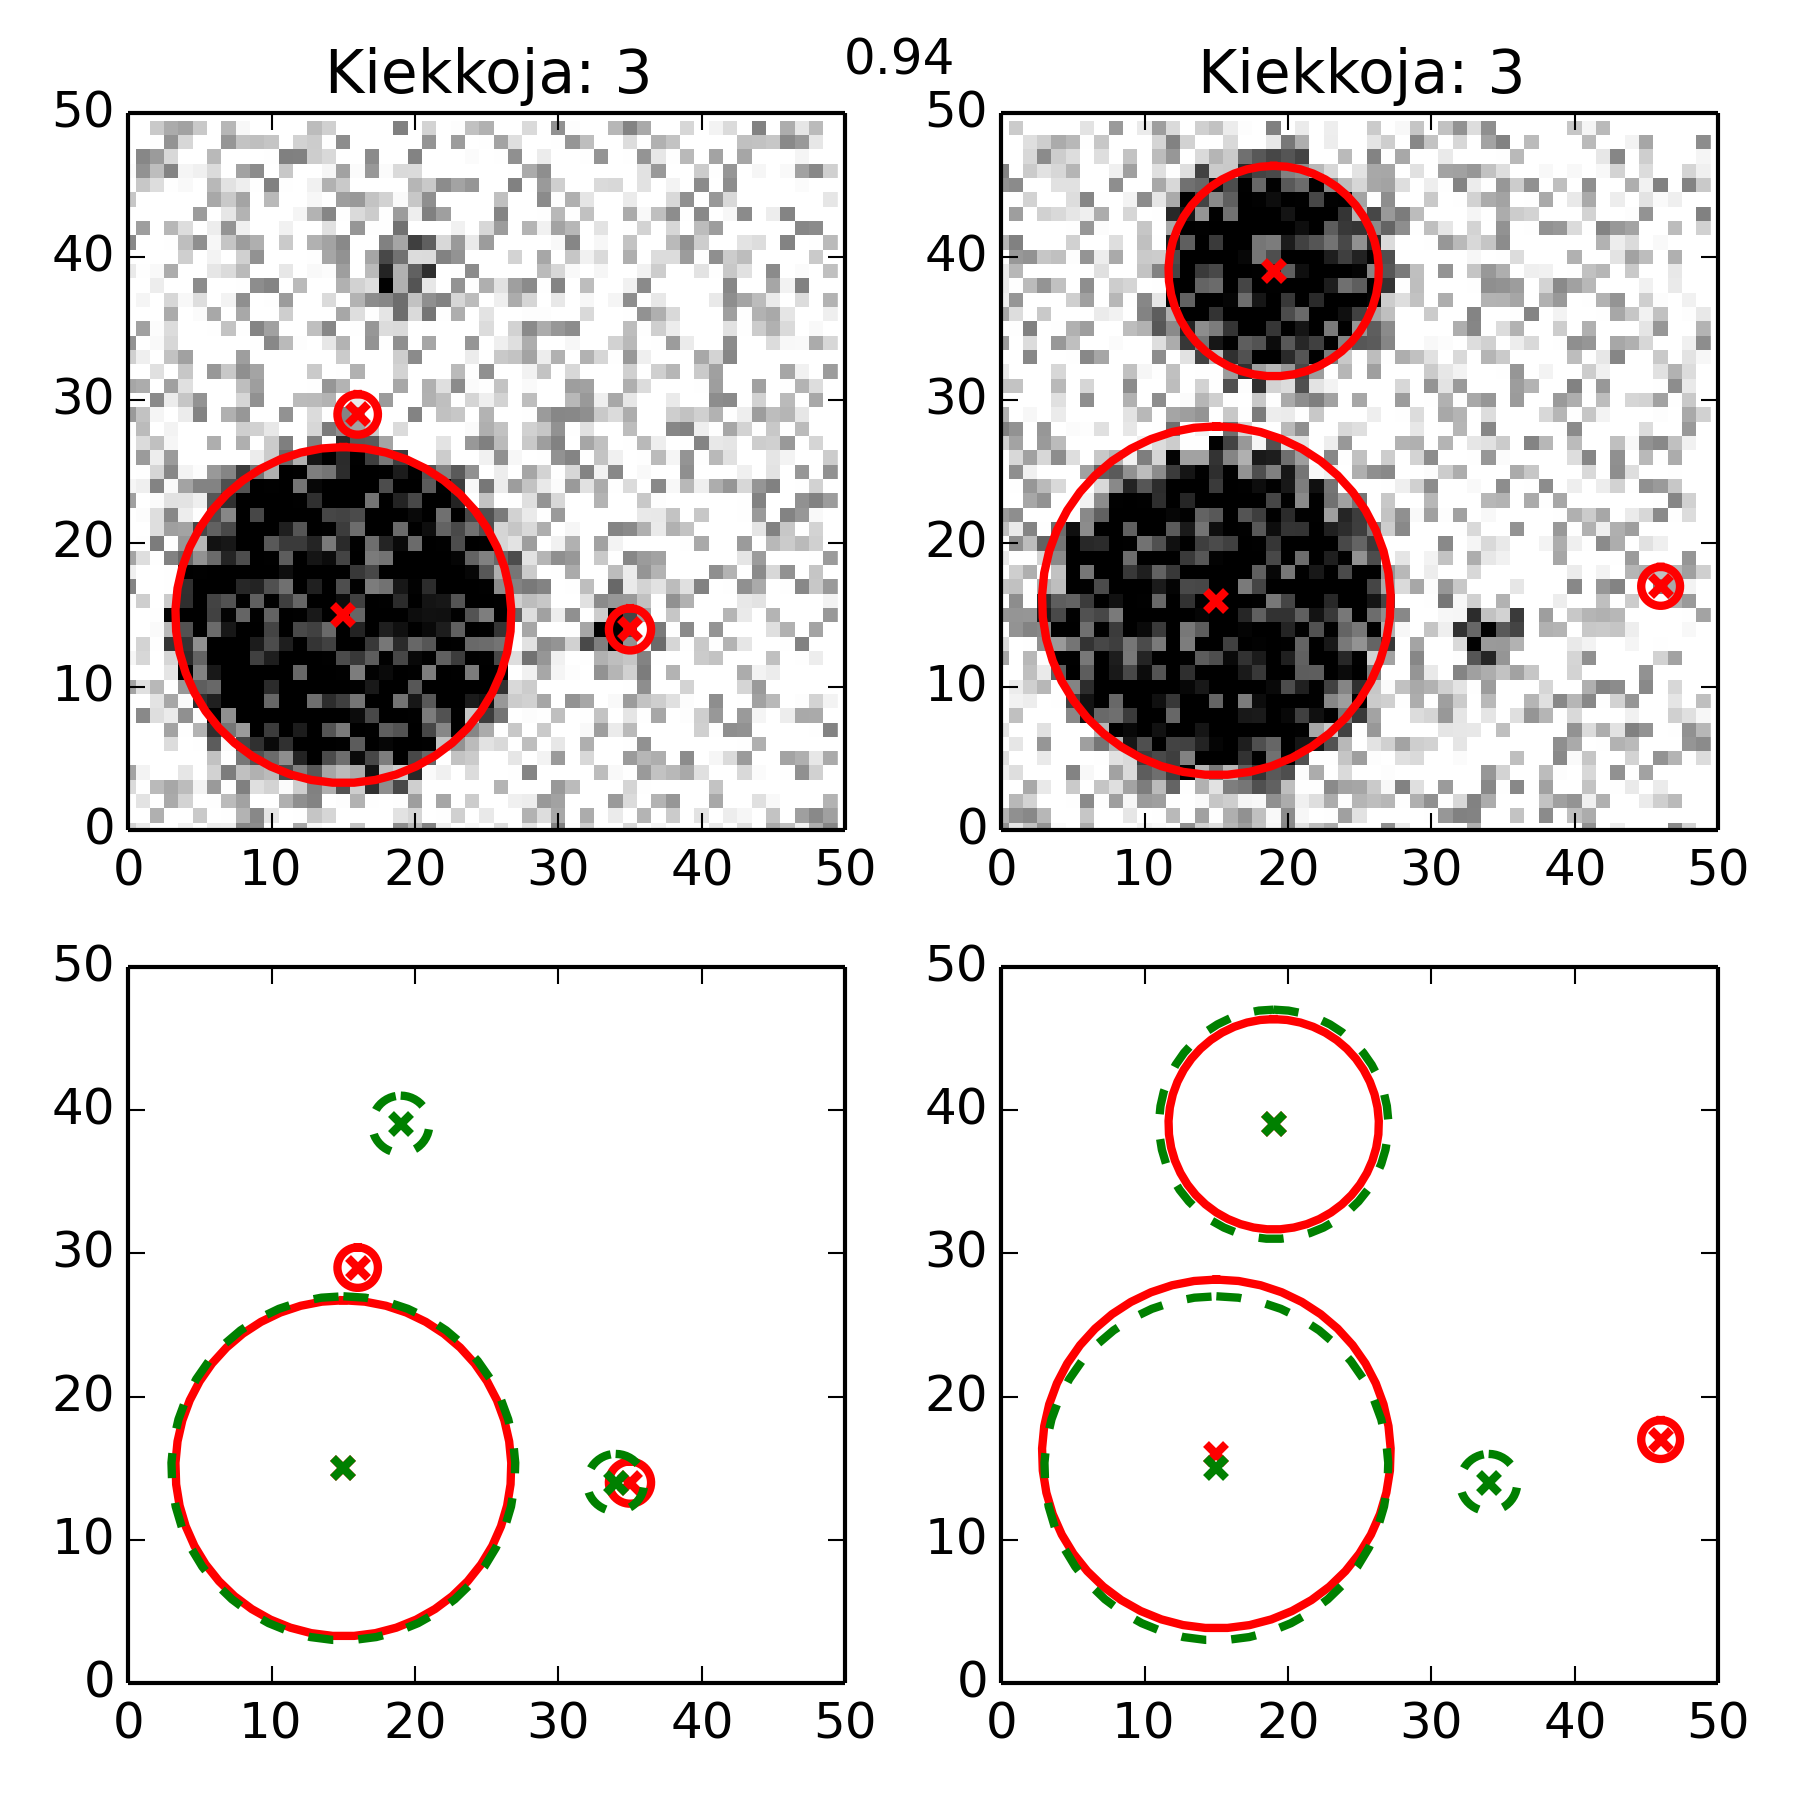
\includegraphics[width=0.7\linewidth]{figures/set3_datasets_res_094.png}
    \caption{
        Testikuvat e, f: Parhaat ratkaisut (punaiset ympyrät) 100 kulkijan kokoelmasta jäähdytysskenaariolla $\alpha = 0.94$.
        \label{fig:set3_datasets_res_094}
    }
\end{figure}


\begin{figure}[htpb]
    \centering
    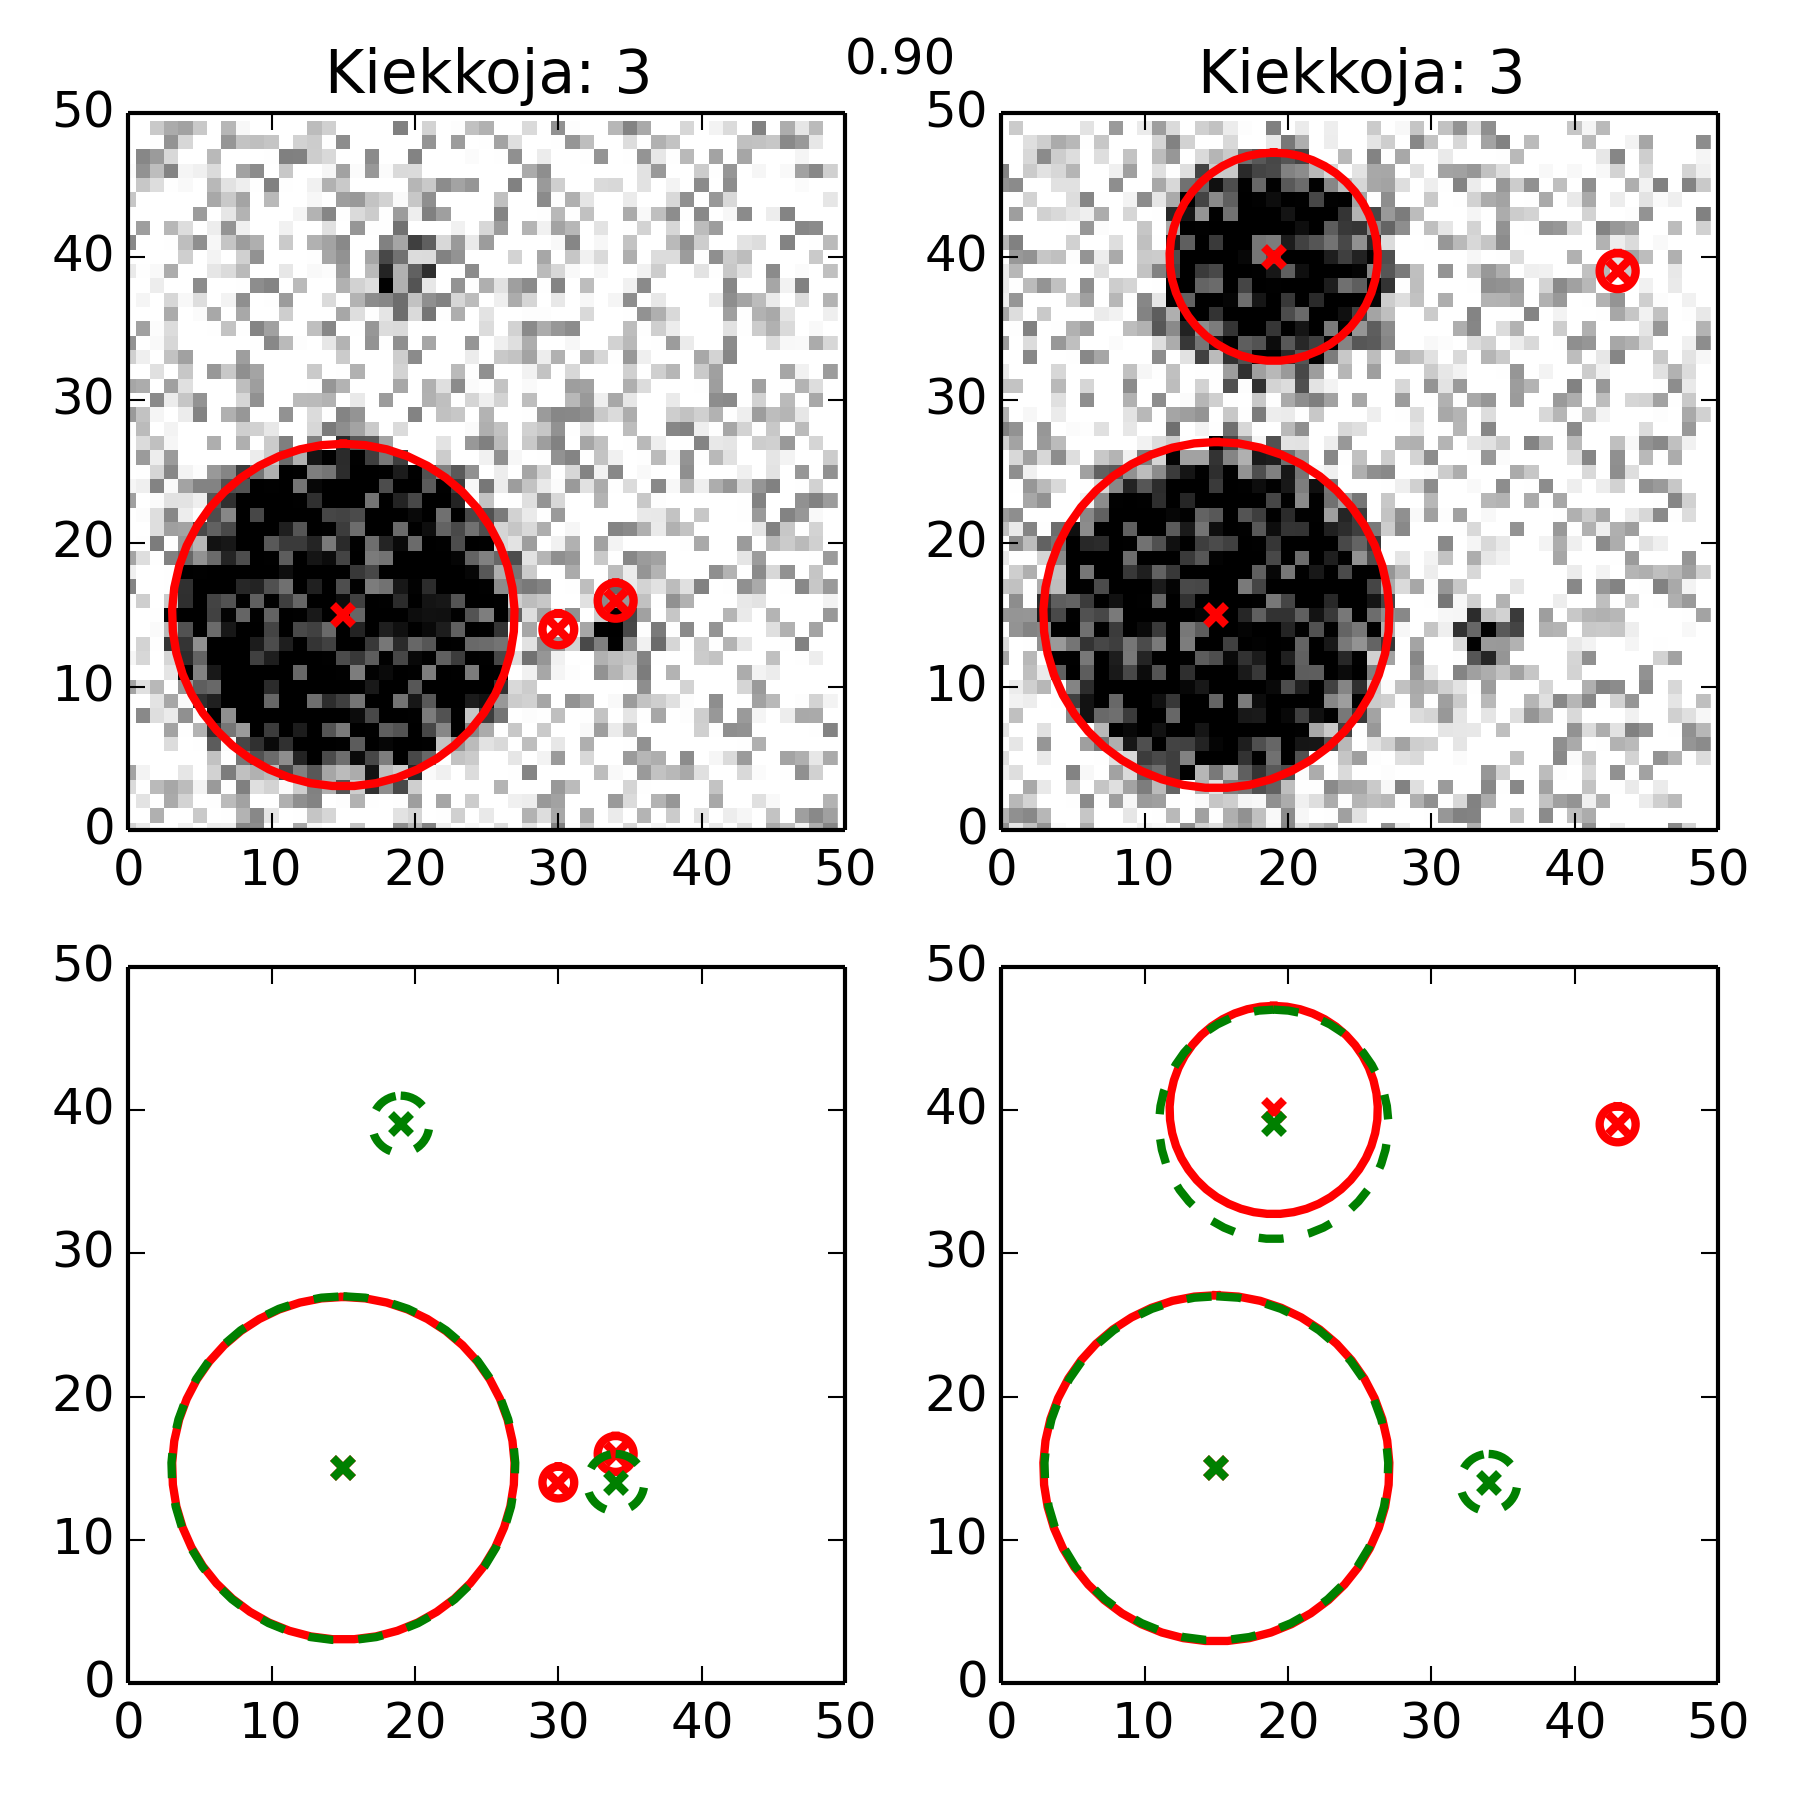
\includegraphics[width=0.7\linewidth]{figures/set3_datasets_res_090.png}
    \caption{
        Testikuvat e, f: Parhaat ratkaisut (punaiset ympyrät) 100 kulkijan kokoelmasta jäähdytysskenaariolla $\alpha = 0.90$.
        \label{fig:set3_datasets_res_090}
    }
\end{figure}


\begin{figure}[htpb]
    \centering
    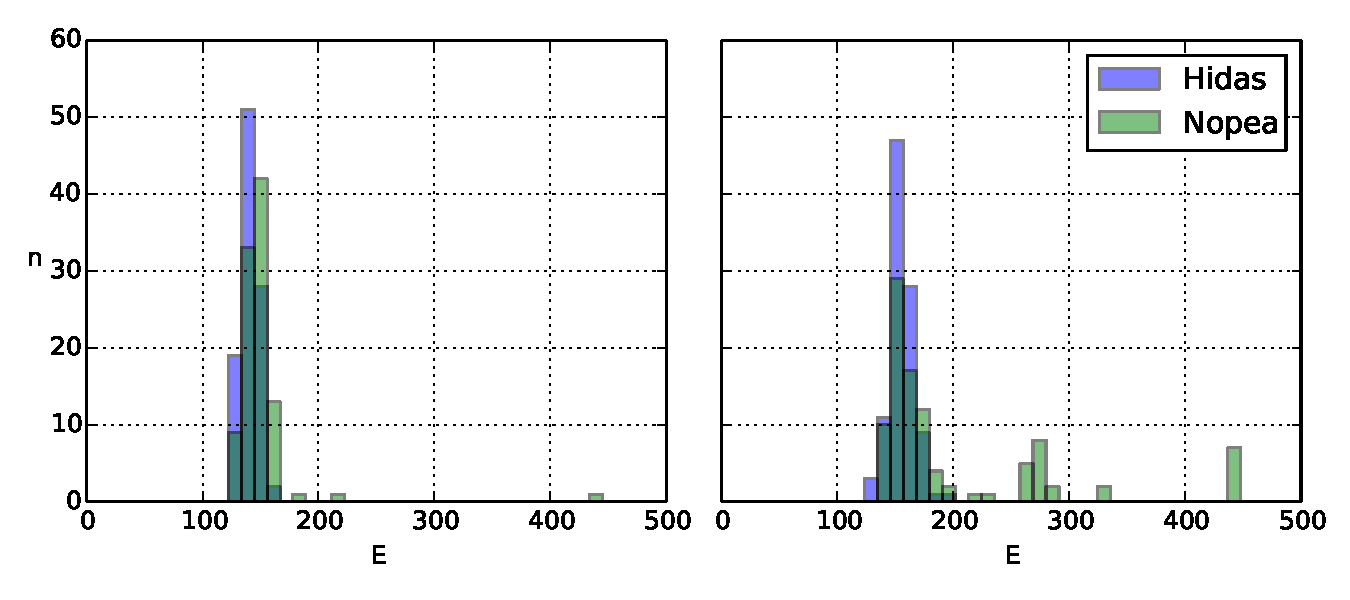
\includegraphics[width=1.0\linewidth]{figures/set3_histo_compare_2_099_090.pdf}
    \caption{Testikuvien e ja f kulkijakokoelmien loppuenergiajakaumien histogrammit jäähdytysskenaarioilla $\alpha = 0.99$ (hidas) ja $\alpha = 0.90$ (nopea)
        \label{fig:set3_histo_compare_2_099_090}
    }
\end{figure}

%Kaikkien kokoelmien lopulliset energiajakaumat. (Loppuenergioiden jakauma)
%
%Kullekin kokoelmalle kaikkein paras energia kulkijoiden määrän funktiona.
%
%Kaikkein parasta energiaa vastaavat ratkaisut.
%
%Niiden virheet.
%
%Tyypillisen / keskimääräisen kävelijän energia ja sitä vastaava ratkaisu.
%
%Graafi kävelijöistä isossa ja pienessä ongelmassa.


